\documentclass{beamer}

\usepackage{beamerthemesplit}
\usepackage{graphicx}
\usepackage{subfigure}
\usepackage{amsmath,amssymb}
\usepackage{multimedia}
\usepackage{times}
\usepackage{ulem}

\usepackage[latin1]{inputenc}
\usepackage[T1]{fontenc}
\usepackage{listings}
\usepackage{courier}
\usepackage{color}
\usepackage{rotating}

\newcommand{\re}{\text{Re}}
\newcommand{\im}{\text{Im}}
\newcommand{\de}{\mbox{d}}
\newcommand{\eref}[1]{(\ref{#1})}
\newcommand{\ii}{\text{i}}
\newcommand{\ee}{\text{e}}
\newcommand{\mathbi}[1]{\textbf{\em #1}}
\newcommand{\rem}[1]{}

\newcommand{\heading}[1]{\centerline{\Large #1} \vspace{0.5em}}
%\newcommand{\heading}[1]{\frametitle{\centerline{#1}}}

\newcommand{\odeint}[0]{odeint}


% Layout specification

% \usetheme{AnnArbor}
% \usetheme{Antibes}
% \usetheme{Bergen}
% \usetheme{Berkeley}
% \usetheme{Berlin}
% \usetheme{Boadilla}
% \usetheme{boxes}
% \usetheme{CambridgeUS}
% \usetheme{Copenhagen}
% \usetheme{Darmstadt}
% \usetheme{default}
% \usetheme{Dresden}
% \usetheme{Frankfurt}
% \usetheme{Goettingen}
% \usetheme{Hannover}
% \usetheme{Ilmenau}
% \usetheme{JuanLesPins}
% \usetheme{Luebeck}
% \usetheme{Madrid}
% \usetheme{Malmoe}
% \usetheme{Marburg}
% \usetheme{Montpellier}
% \usetheme{PaloAlto}
% \usetheme{Pittsburgh}
% \usetheme{Rochester}
% \usetheme{Singapore}
% \usetheme{Szeged}
\usetheme{Warsaw}

% \usecolortheme{albatross}
% \usecolortheme{beaver}
% \usecolortheme{beetle}
% \usecolortheme{crane}
% \usecolortheme{default}
% \usecolortheme{dolphin}
% \usecolortheme{dove}
% \usecolortheme{fly}
% \usecolortheme{lily}
% \usecolortheme{orchid}
% \usecolortheme{rose}
% \usecolortheme{seagull}
% \usecolortheme{seahorse}
% \usecolortheme{sidebartab}
% \usecolortheme{structure}
% \usecolortheme{whale}
% \usecolortheme{wolverine}

% \usefonttheme{default}
% \usefonttheme{professionalfonts}
% \usefonttheme{serif}
% \usefonttheme{structurebold}
% \usefonttheme{structureitalicserif}
% \usefonttheme{structuresmallcapsserif}

% \useinnertheme{circles}
% \useinnertheme{default}
% \useinnertheme{inmargin}
% \useinnertheme{rectangles}
% \useinnertheme{rounded}

% \useoutertheme{default}
% \useoutertheme{infolines}
% \useoutertheme{miniframes}
% \useoutertheme{shadow}
% \useoutertheme{sidebar}
% \useoutertheme{smoothbars}
% \useoutertheme{smoothtree}
% \useoutertheme{split}
% \useoutertheme{tree}



% Meta

\title[odeint]{Solving ODEs with CUDA and OpenCL}
\subtitle[odeint]{using Boost.Odeint}
\author[Karsten Ahnert]{Karsten Ahnert$^{1,2}$ and Mario Mulansky$^2$}
\institute[Universit\"at Potsdam]{$^1$ Ambrosys GmbH, Potsdam\\ $^2$ Institut f\"ur Physik und Astronomie, Universit\"at Potsdam}
\date{Februar 2, 2013}
%\logo{\pgfimage[width=2cm,height=2cm]{logo}}
\titlegraphic{\includegraphics[width=4cm]{ambrosys}\hspace{5ex}
\includegraphics[width=1.5cm,height=1.5cm]{logo}\hspace{7ex}}
\subject{Subject}
\keywords{Keyword1,Keyword2}



\definecolor{dark-gray}{gray}{0.15}
\definecolor{light-gray}{gray}{0.8}
\definecolor{lighter-gray}{gray}{0.9}

\definecolor{dark-green}{rgb}{0,0.4,0}
\definecolor{dark-red}{rgb}{0.2,0,0}

\newcommand{\highlight}[1]{\bf #1}

\lstset{
         basicstyle=\small\ttfamily, % Standardschrift
         %numbers=left,               % Ort der Zeilennummern
         numberstyle=\tiny,          % Stil der Zeilennummern
         %stepnumber=2,               % Abstand zwischen den Zeilennummern
         numbersep=0pt,              % Abstand der Nummern zum Text
         tabsize=2,                  % Groesse von Tabs
         extendedchars=true,         %
         breaklines=true,            % Zeilen werden Umgebrochen
         frame=single,         
         backgroundcolor=\color{lighter-gray},
         tabsize=2,
         keywordstyle=\color{dark-green},
         identifierstyle=,
         commentstyle=\color{dark-gray}\normalfont\rmfamily\itshape,
         stringstyle=\color{dark-red},
         showspaces=false,           % Leerzeichen anzeigen ?
         showtabs=false,             % Tabs anzeigen ?
         xleftmargin=10pt,
         xrightmargin=10pt,
         framexleftmargin=5pt,
         framexrightmargin=5pt,
         framexbottommargin=4pt,
         language=c++,
         showstringspaces=false      % Leerzeichen in Strings anzeigen ?        
 }
\lstloadlanguages{C++}


% What is shown

\beamertemplatenavigationsymbolsempty
  \setbeamertemplate{footline}{}
%\setbeamertemplate{footline}{\insertframenumber}
\setbeamertemplate{headline}{}


\parindent0pt











\begin{document}



\frame{
  \titlepage
}

\rem{
\begin{frame}
  \heading{Outline}

  \tableofcontents
\end{frame}
}


\begin{frame}
 \heading{Introduction}

 \begin{itemize}
  \item Solve large systems of coupled ODEs
  \item Use odeint - Boost Library
  \item Compare several open source frameworks for GPGPU computation
  \item VexCL, ViennaCL, Thrust, MTL
 \end{itemize}

\end{frame}


\begin{frame}
 
\heading{What is an ODE? -- Examples}

\vspace{2ex}

\begin{minipage}{0.48\textwidth}
 \begin{center}
  Newtons equations

  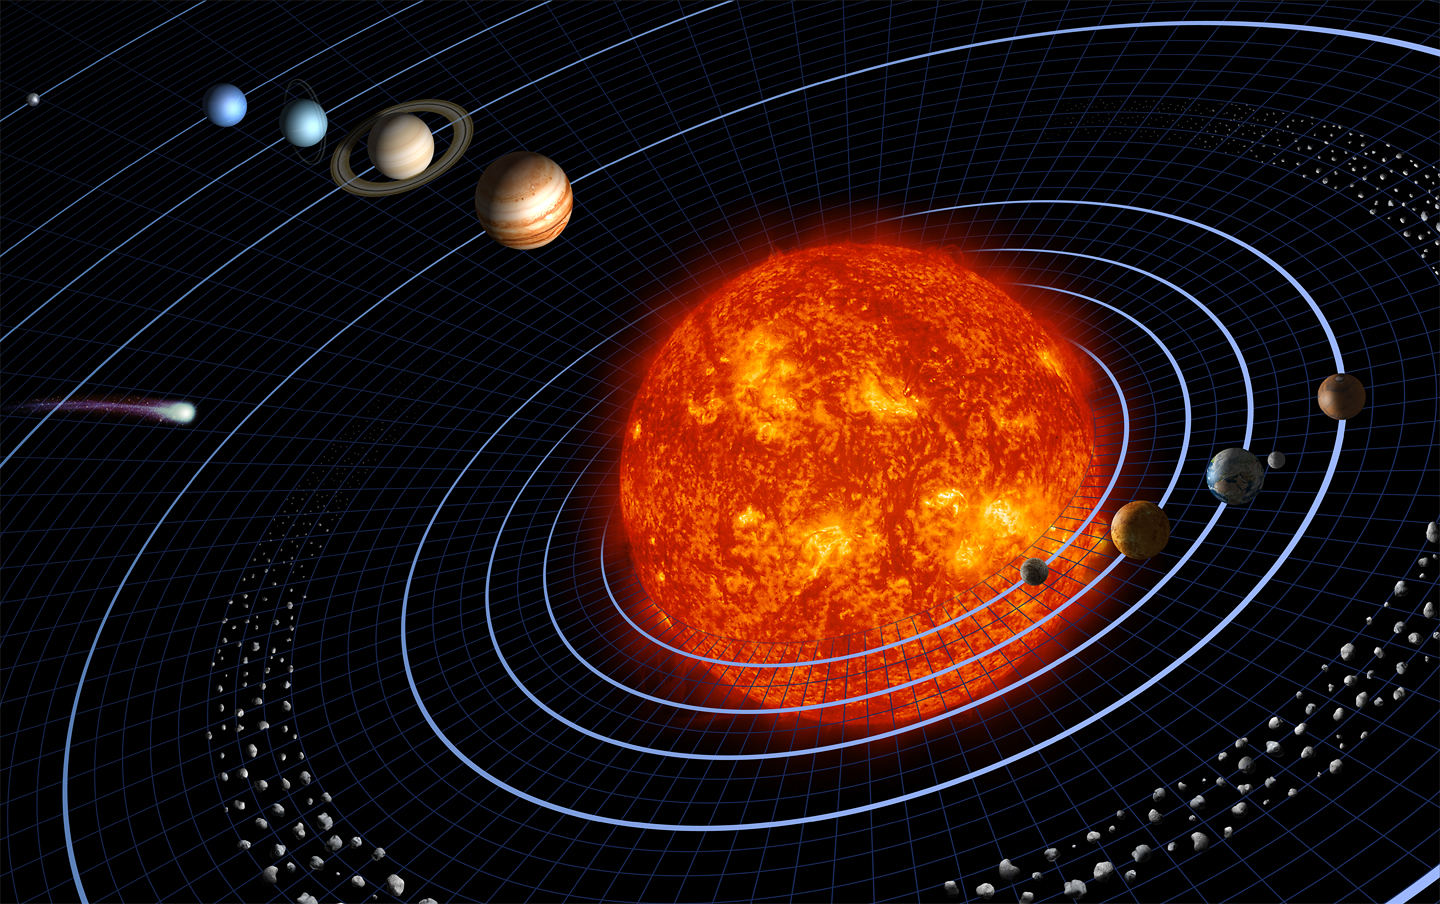
\includegraphics[draft=false,width=0.8\textwidth]{solar_system.jpg}
 \end{center}
\end{minipage}
%\pause
\begin{minipage}{0.48\textwidth}
 \begin{center}
  Reaction and relaxation equations (i.e. blood alcohol content, chemical reaction rates)
 \end{center}
\end{minipage}
%\pause
\vspace{2ex}

\begin{minipage}{0.48\textwidth}
 \begin{center}
  Granular systems

  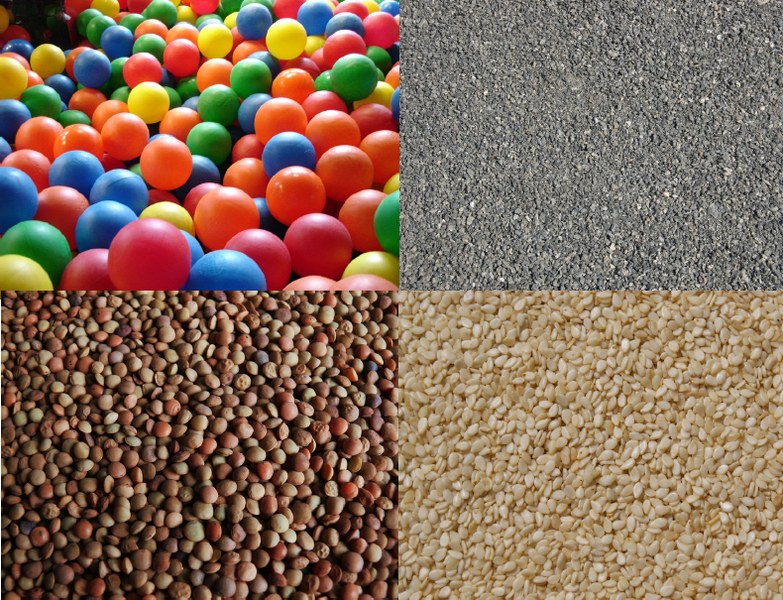
\includegraphics[draft=false,width=0.65\textwidth]{granular_system.png}
 \end{center}
\end{minipage}
%\pause
\begin{minipage}{0.48\textwidth}
 \begin{center}
  Interacting neurons

  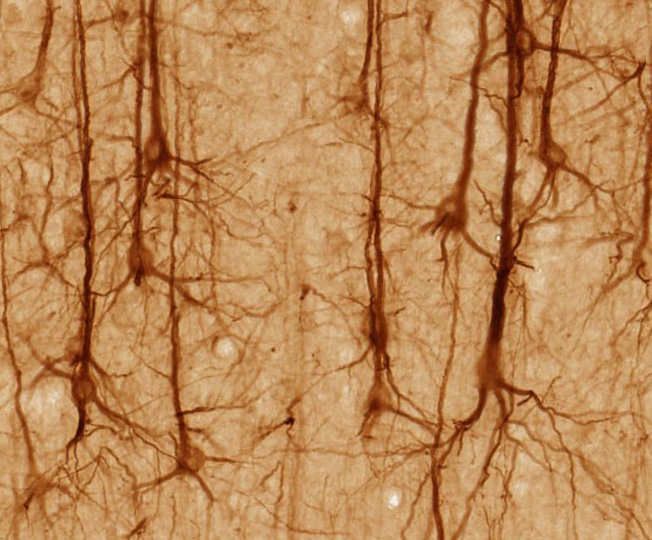
\includegraphics[draft=false,width=0.6\textwidth]{neuron.jpg}
 \end{center}
\end{minipage}
%\pause
\vspace{2ex}

\begin{itemize}
 \item Many examples in physics, biology, chemistry, social sciences
 \item Fundamental in mathematical modelling
\end{itemize}

\end{frame}



\begin{frame}
 
 \heading{What is an ODE?}

 $$\frac{\de x(t)}{\de t} = f\big(x(t) , t\big) \qquad \qquad {\scriptsize \text{short form}} \qquad \dot{x} = f(x,t)
$$

 \begin{itemize}
  \item $x(t)$ -- dependent variable
  \item $t$ -- indenpendent variable (time)
  \item $f(x,t)$ -- defines the ODE
 \end{itemize}

\vspace{4ex}

 Initial Value Problem (IVP):

 $$\dot x = f( x , t ) ,\qquad x(t=0) = x_0$$

\end{frame}


\begin{frame}
  
 \heading{Numerical integration of ODEs}
  
\vspace{4ex}
    Find a numerical solution of an ODE and its IVP
    \[ \dot{x} = f(x,t) \,\,\textrm{,} \quad \quad x(t=0) = x_0\]

   \vspace{2ex}

   Example: Explicit Euler
   \[ x(t + \Delta t ) = x(t) + \Delta t \,\cdot\, f(x(t),t) + \mathcal{O}(\Delta t^2)\]

   \vspace{2ex}

   General scheme of order $s$
    \[ x(t) \,\, \mapsto \,\, x(t+\Delta t) \quad \quad \text{, or}\]
    \[x(t + \Delta t) = \mathcal{F}_t x(t) + \mathcal{O}(\Delta t^{s+1})\]

\end{frame}





\begin{frame}[fragile]

 \heading{Algebras and operations}

 \vspace{2ex}

Euler method

$$\text{for all i :}  \quad \quad x_i(t+\Delta t) = x_i(t) + \Delta t \cdot f_i(x)$$

\vspace{2ex}

\begin{lstlisting}
typedef euler< state_type ,
   value_type , deriv_type , time_type,
   algebra , operations , resizer > stepper; 
\end{lstlisting}


\begin{itemize}
\item Algebras perform the iteration over $i$.
\item Operations perform the elementary addition.
\end{itemize}

\vspace{2ex}

Usage:

\begin{lstlisting}
  stepper s;
  s.do_step( ode , x , t , dt );
\end{lstlisting}

\end{frame}













\begin{frame}[fragile]
 \heading{Algebras and operations}

\vspace{1ex}
Algebra has to have defined the following member functions:

\begin{itemize}
 \item \lstinline+algebra.for_each1( x1 , unary_operation );+
 \item \lstinline+algebra.for_each2( x1, x2, binary_operation );+
 \item ...
\end{itemize}

\vspace{2ex}

\lstinline+Operations+ is a class with the following (static) functors:
\begin{itemize}
 \item \lstinline+scale_sum1       // calculates y = a1*x1+
 \item \lstinline{scale_sum2       // calculates y = a1*x1 + a2*x2}
 \item ...
\end{itemize}

\vspace{2ex}
\begin{lstlisting}
algebra.for_each3( x1 , x0 , F1 ,
   Operations::scale_sum2( 1.0, b1*dt );
\end{lstlisting}

This computes: $\vec x_1 = 1.0\cdot \vec x_0 + b_1\Delta t\cdot \vec F_1$.
\end{frame}




\begin{frame}[fragile]
 \heading{Algebra and operations}

 \begin{itemize}
  \item {\tt range\_algebra} -- Default algebra, supporting Boost.Range
  \item {\tt default\_operations} -- Default operations
  \item {\tt vector\_space\_algebra} -- Types with vector space
    semantic, i.e. \lstinline{y = a1*x1 + a2*x2}. Can be used by all
    types supporting expression templates.
  \item {\tt thrust\_algebra}, {\tt thrust\_operations} -- Thrust's device vectors
 \end{itemize}

\end{frame}




\begin{frame}[fragile]
 \heading{GPU Frameworks}

\begin{itemize}
 \item VexCL - Vector Expression Framework, Sparse matrix support
 \item ViennaCL - Linear algebra framework - not restricted to OpenCL
 \item Thrust - general purpose algorithm library, mimicks the STL interface for CUDA devices
 \item MTL4 - Matrix template libary
\end{itemize}

\end{frame}



\begin{frame}[fragile]
 \heading{Example - Parameter study of Lorenz system}

\begin{eqnarray*}
\dot{x} & = & - \sigma ( y - x ) \\
\dot{y} & = & R x - y - x z \\
\dot{z} & = & - b z + x y
\end{eqnarray*}

Dependence of chaoticity on parameter $R$

\vspace{2ex}

Solve many ODE in parallel $x_i,y_i,z_i,R_i$

\end{frame}


\begin{frame}[fragile]
 \heading{VexCL}

\begin{lstlisting}[basicstyle=\scriptsize\ttfamily]
typedef vex::vector< value_type >    vector_type;
typedef vex::multivector< value_type, 3 > state_type;

struct sys_func
{
  const vector_type &R;
  sys_func( const vector_type &_R ) : R( _R ) { }
  void operator()(
    const state_type &x, state_type &dxdt, value_type t)
  {
    dxdt = std::tie( sigma * (x(1) - x(0)) ,
                     R * x(0) - x(1) - x(0) * x(2),
                     x(0) * x(1) - b * x(2) );
  }
};

odeint::runge_kutta4<
  state_type , value_type , state_type , value_type ,
  odeint::vector_space_algebra , odeint::default_operations
  > stepper;

odeint::integrate_const( stepper , sys_func( R ) , X , value_type(0.0) , t_max , dt );

\end{lstlisting}

\end{frame}



\begin{frame}[fragile]
 \heading{ViennaCL}

show code

\end{frame}




\begin{frame}[fragile]
 \heading{Thrust}

 show code
\end{frame}


\begin{frame}[fragile]
 \heading{MTL4}

 show code

\end{frame}


\begin{frame}[fragile]
 \heading{Performance}

 show picture
\end{frame}

\begin{frame}[fragile]
 \heading{Conclusion}

 \begin{itemize}
  \item Usability - they differ
  \item Performance - they are equal more or less
  \item Optimize by hand
 \end{itemize}

 Programming CUDA and OpenCL: A Case Study Using Modern C++ Libraries. Denis Demidov, Karsten Ahnert, Karl Rupp, Peter Gottschling. arXiv:1212.6326.

\end{frame}





\rem{
\section{Introduction}


\rem{
\begin{frame}
 
 \only<1>{

   \heading{{\color{red}\bf ode}int}

   \vspace{6ex}

   \Large

   ode \hspace{4ex} ordinary differential equation

   \vspace{5ex}

}

 \only<2>{
   \heading{ode{\color{red}\bf int}}

   \vspace{6ex}

   \Large

   ode \hspace{4ex} ordinary differential equation

   \vspace{3ex}

   int \hspace{4ex} integration
}

\end{frame}
}


\begin{frame}
 
\heading{What is an ODE? -- Examples}

\vspace{2ex}

\begin{minipage}{0.48\textwidth}
 \begin{center}
  Newtons equations

  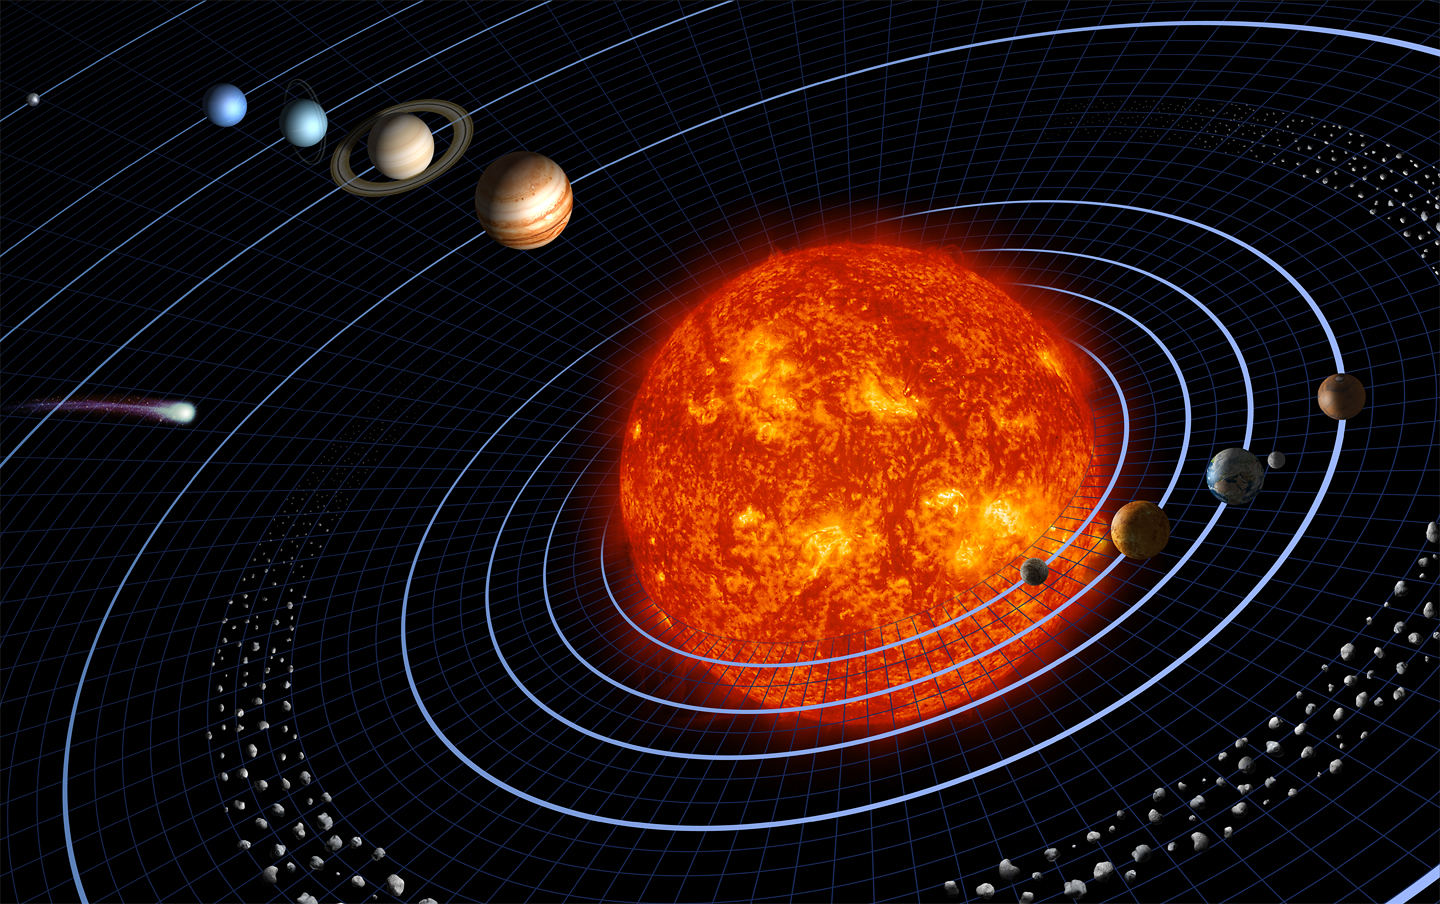
\includegraphics[draft=false,width=0.8\textwidth]{solar_system.jpg}
 \end{center}
\end{minipage}
\begin{minipage}{0.48\textwidth}
 \begin{center}
  Reaction and relaxation equations (i.e. blood alcohol content)
 \end{center}
\end{minipage}

\vspace{2ex}

\begin{minipage}{0.48\textwidth}
 \begin{center}
  Granular systems

  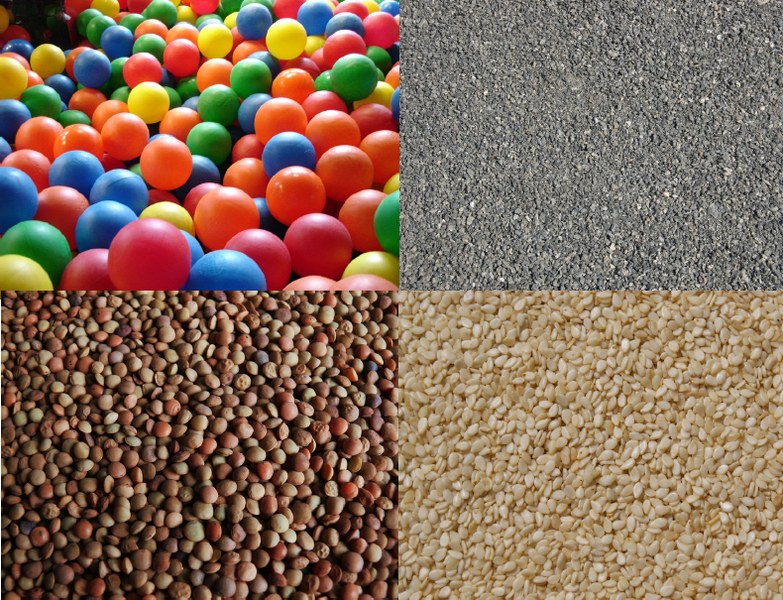
\includegraphics[draft=false,width=0.65\textwidth]{granular_system.png}
 \end{center}
\end{minipage}
\begin{minipage}{0.48\textwidth}
 \begin{center}
  Interacting neurons

  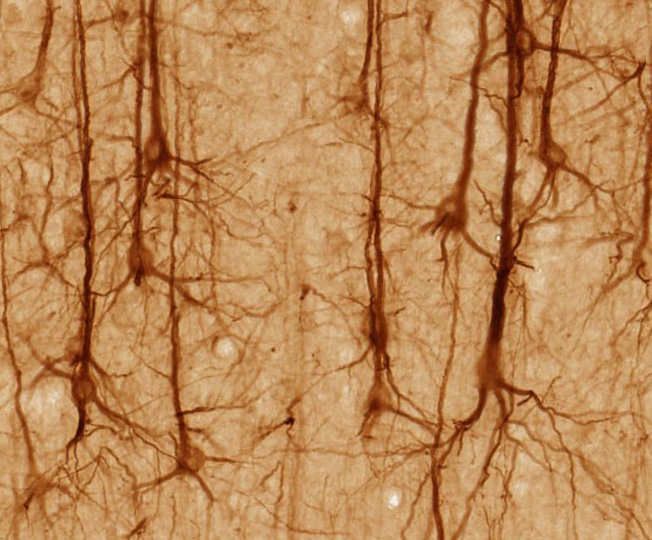
\includegraphics[draft=false,width=0.6\textwidth]{neuron.jpg}
 \end{center}
\end{minipage}

\vspace{2ex}

\begin{itemize}
 \item Many examples in physics, biology, chemistry, social sciences
 \item Fundamental in mathematical modelling
\end{itemize}

\end{frame}



\begin{frame}
 
 \heading{What is an ODE?}

 $$\frac{\de x(t)}{\de t} = f\big(x(t) , t\big) \qquad \qquad {\scriptsize \text{short form}} \qquad \dot{x} = f(x,t)
$$

 \begin{itemize}
  \item $x(t)$ -- dependent variable
  \item $t$ -- indenpendent variable (time)
  \item $f(x,t)$ -- defines the ODE
 \end{itemize}

\vspace{4ex}

 Initial Value Problem (IVP):

 $$\dot x = f( x , t ) ,\qquad x(t=0) = x_0$$

 \centerline{Find $x(t)$}

\end{frame}


\begin{frame}
  
 \heading{Numerical integration of ODEs}
  
\vspace{4ex}
    Find a numerical solution of an ODE an its initial value problem 
    \[ \dot{x} = f(x,t) \,\,\textrm{,} \quad \quad x(t=0) = x_0\]

   \vspace{2ex}

   Example: Explicit Euler
   \[ x(t + \Delta t ) = x(t) + \Delta t \,\, f(x(t),t) + \mathcal{O}(\Delta t^2)\]

   \vspace{2ex}

   General scheme of order $s$
    \[ x(t) \,\, \mapsto \,\, x(t+\Delta t) \quad \quad \text{, or}\]
    \[x(t + \Delta t) = \mathcal{F}_t x(t) + \mathcal{O}(\Delta t^{s+1})\]

\end{frame}




\frame{
%  \frametitle{odeint - Solving ODEs in C++}

\heading{\bf \color{red}odeint}

\vspace{2ex}

\centerline{Solving ordinary differential equations in C++}

\vspace{2ex}

Open source
\begin{itemize}
\item Boost license -- do whatever you want do to with it 
\end{itemize}

\pause

\vspace{2ex}

Download
\begin{itemize}
\item \texttt{\textbf{www.odeint.com}}
% \item \texttt{https://github.com/headmyshoulder/odeint-v2}
\end{itemize}

\pause

\vspace{2ex}

Modern C++
\begin{itemize}
 \item Generic programming, functional programming 
 \item Fast, easy-to-use and extendable.
 \item Container independent
 \item Portable
\end{itemize}

}





\begin{frame}[fragile]
 
 \heading{Who uses odeint}

\vspace{4ex}



\begin{minipage}{0.2\textwidth}
 \begin{center}
  NetEvo

  \vspace{1ex}
  
  
\includegraphics[draft=false,width=1.0\textwidth]{netevo.png}
 \end{center}
\end{minipage}
\hspace{4ex}\begin{minipage}{0.4\textwidth}
 \begin{center}
  OMPL -- Open Motion Planning Library
 \end{center}
\end{minipage}


\end{frame}





\begin{frame}
  \heading{Motivation: The interface problem in C/C++}

  \vspace{2ex}
  
    \begin{itemize}
      \item Many frameworks exist to do numerical computations.
      \item Data has to be stored in containers or collections.
      \item GSL: {\tt gsl\_vector}, {\tt gsl\_matrix}
      \item NR: pointers with Fortran-style indexing
      \item Blitz++, MTL4, boost::ublas
      \item QT: {\tt QVector}, wxWidgets: {\tt wxArray}, MFC: {\tt CArray}
    \end{itemize}

  %\vspace{2ex}

    {\bf \color{red} But:} All books on C++ recommend the use of the STL containers {\tt std::vector},
    {\tt std::list}, \dots

 \pause

  %\vspace{2ex}

  \begin{block}{Theoretical solution of the interface mess}
  GoF Design Pattern: Adaptor, also known as Wrapper
  \end{block}

  \pause

  \begin{exampleblock}{Alternative}
   Generic, container independent algorithms
  \end{exampleblock}

\end{frame}



\begin{frame}
  
  \heading{Portability of your algorithm}

  \vspace{1ex}

  How to run your algorithm?
    \begin{itemize}
      \item Single machine, single CPU
      \item Single machine, multiple CPU's (OpenMP, threads, ...)
      \item Multiple machines (MPI)
      \item GPU (Cuda, Thrust, OpenCL)
    \end{itemize}

  \pause

  \vspace{1ex}

  Which data types are used by your algorithm?
   \begin{itemize}
    \item Build-in data types -- \texttt{double}, \texttt{complex<double>}
    \item Arbitrary precision types -- GMP, MPFR
    \item Vectorial data types \texttt{float2d}, \texttt{float3d}
   \end{itemize}

  \pause

  \vspace{1ex}

  \begin{block}{Theoretical solution}
    GoF Design Pattern: Strategy, also known as Policy
  \end{block}

  \begin{exampleblock}{Alternative}
   Generic algorithms
  \end{exampleblock}

\end{frame}




\section{Tutorial}



\begin{frame}
  \heading{Let's step into \odeint}
  \tableofcontents[currentsection] 
\end{frame}


\begin{frame}[fragile]

\heading{Example -- Pendulum}

\vspace{2ex}

\begin{columns}[T]
  \begin{column}{0.35\textwidth}
    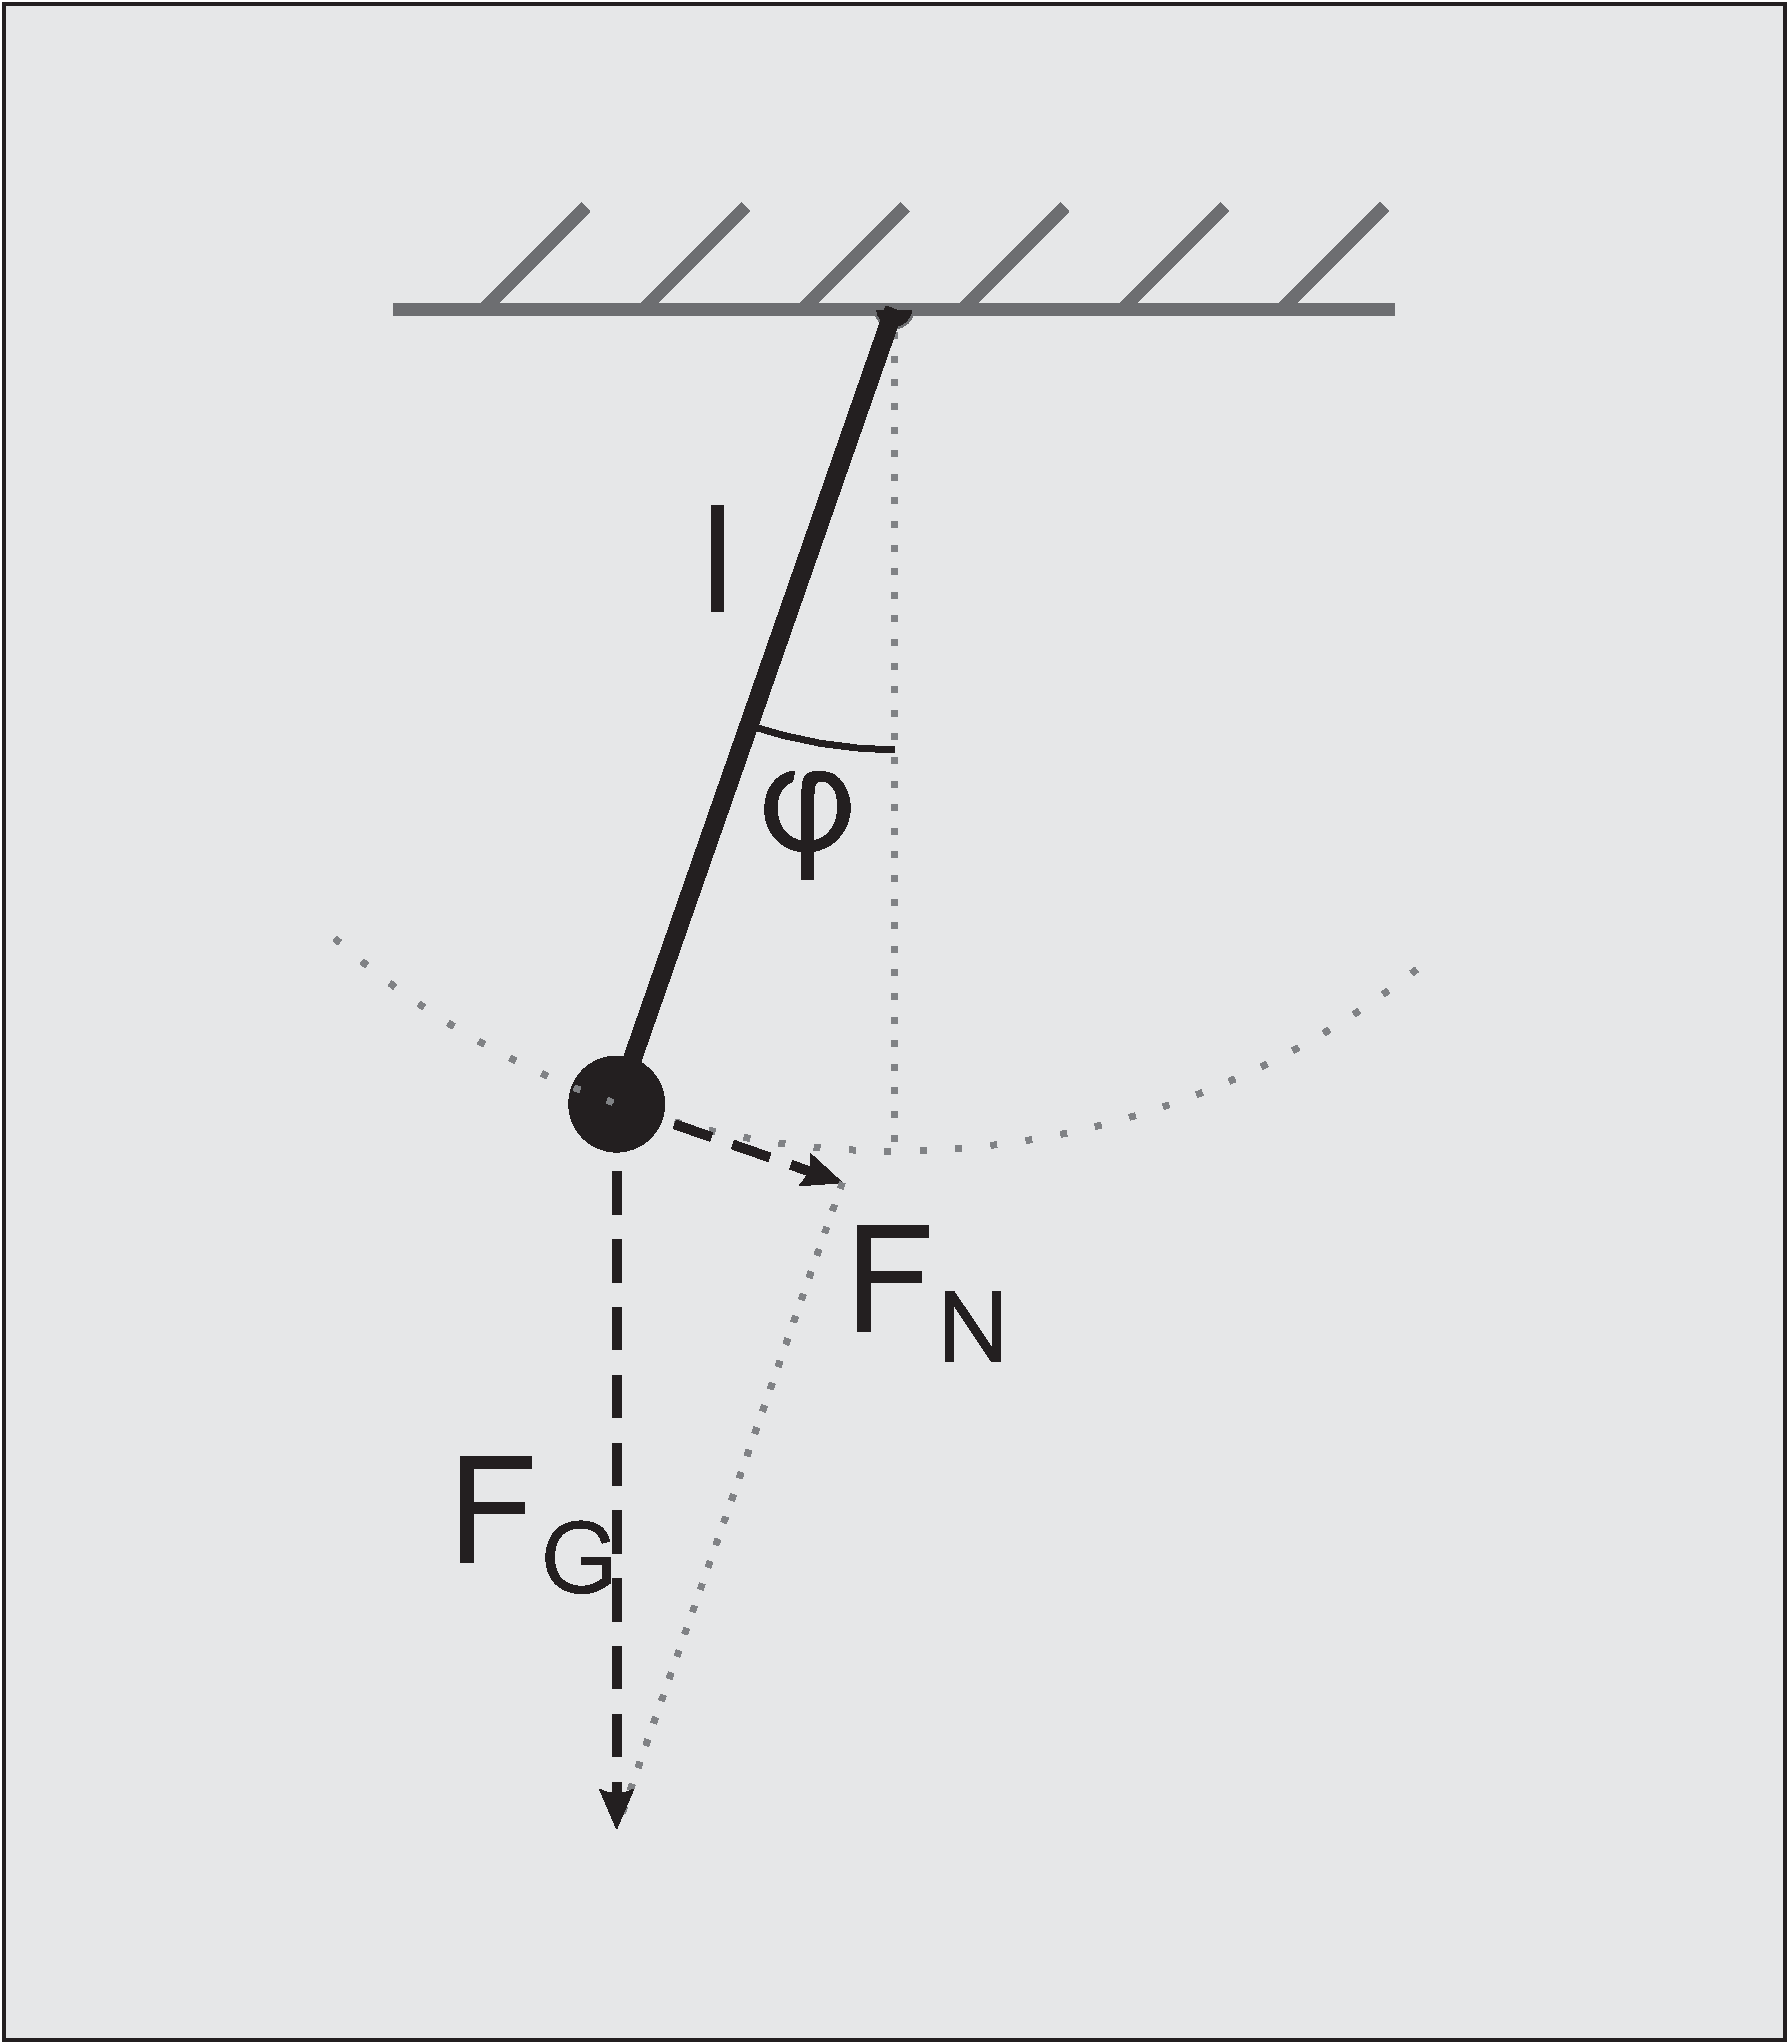
\includegraphics[draft=false,width=1.0\textwidth]{pendulum.pdf}

   \vspace{4ex}
  \end{column}

  \begin{column}{0.65\textwidth}
 \only<1>{
 Newtons law: $m a = F$

 \vspace{2ex}

 Acceleration:  $a = l \ddot{\varphi} = \frac{\de^2 \varphi}{\de t^2} $

 \vspace{2ex}

 Force: $F=F_N = - m g \sin \varphi$

 \vspace{4ex}

 $\Longrightarrow$ {\bf ODE for $\varphi$}

 $$\ddot{\varphi} = - g / l \sin \varphi = -\omega_0^2 \sin \varphi$$
 }

 \only<2>
 {

 $$\ddot{\varphi} = - \omega_0^2 \sin \varphi $$

 Small angle: $\sin \varphi \approx \varphi$

 \vspace{2ex}

 Harmonic oscillator $\ddot{\varphi} = - \omega_0^2 \varphi$

 \vspace{2ex}

 Analytic solution: $\varphi = A \cos \omega_0 t + B \sin \omega_0 t$

 \vspace{2ex}

 Determine $A$ and $B$ from initial condition\rem{:

 \centerline{$\varphi(t=0) = \varphi_0 \,\, \text{,} \quad \dot{\varphi}(t=0) = \dot{\varphi}_0$}

 \centerline{$B=\varphi_0 \,\, \text{,} \quad A=\dot{\varphi}_0 / \omega$}}

 }

 \only<3>{

 Full equation: $\ddot{\varphi} = -\omega_0^2 \sin \varphi $

 \vspace{2ex}

 Pendulum with friction and external driving:

 $$\ddot{\varphi} = -\omega_0^2 \sin \varphi - \mu \dot{\varphi} + \varepsilon \sin \omega_E t $$

 \vspace{2ex}

 No analytic solution is known

 \vspace{2ex}

 $\Longrightarrow$ {\bf Solve this equation numerically.}

 }

 \only<4>{

 $$\ddot{\varphi} = -\omega_0^2 \sin \varphi - \mu \dot{\varphi} + \varepsilon \sin \omega_E t $$

 \vspace{2ex}

 Create a first order ODE

 \vspace{1ex}

 \centerline{$x_1 = \varphi \,\, \text{,} \quad x_2 = \dot{\varphi}$}

 \vspace{-3ex}
 \begin{align*}
   \dot{x_1} &= x_2 \\
   \dot{x_2} &= - \omega_0  \sin x_1 - \mu x_2 + \varepsilon \sin \omega_E t  
 \end{align*}


 $x_1$ and $x_2$ are the state space variables

 }
   
  \end{column}
\end{columns}

 

\end{frame}







\begin{frame}[fragile]

\centerline{ \Large Let's solve the pendulum example numerically}

\vspace{2ex}
\begin{lstlisting}
#include <boost/numeric/odeint.hpp>

namespace odeint = boost::numeric::odeint;
\end{lstlisting}

\vspace{2ex}

\centerline{$\dot{x_1} = x_2 \,\,\text{,} \quad \dot{x_2} = - \omega_0 \sin x_1 - \mu x_2 + \varepsilon \sin \omega_E t$}

\vspace{2ex}
\begin{lstlisting}
typedef std::array<double,2> state_type;
\end{lstlisting}

\end{frame}

\begin{frame}[fragile]

\centerline{ \Large Let's solve the pendulum example numerically}

\vspace{2ex}

$\dot{x_1} = x_2$, $\dot{x_2} = - \omega_0^2 \sin x_1 - \mu x_2 + \varepsilon \sin \omega_E t$ \hspace{6ex} $\omega_0^2 = 1$

\vspace{2ex}

\begin{lstlisting}
struct pendulum
{
  double m_mu, m_omega, m_eps;

  pendulum(double mu,double omega,double eps)
  : m_mu(mu),m_omega(omega),m_eps(eps) { }

  void operator()(const state_type &x,state_type &dxdt,double t) const
  {
    dxdt[0] = x[1];
    dxdt[1] = -sin(x[0]) - m_mu * x[1] +
        m_eps * sin(m_omega*t);
  }
};
\end{lstlisting}

\end{frame}

\begin{frame}[fragile]
 \centerline{ \Large Let's solve the pendulum example numerically}

\vspace{2ex}
$\varphi(0) = x_1(0) = 1 \,\, \text{,} \quad \dot{\varphi}(0) = x_2(0) = 0$
\vspace{2ex}

\begin{lstlisting}
odeint::runge_kutta4< state_type > rk4;
pendulum p( 0.1 , 1.05 , 1.5 );

state_type x = {{ 1.0 , 0.0 }};
double t = 0.0;

const double dt = 0.01;
rk4.do_step( p , x , t , dt );
t += dt;
\end{lstlisting}

\vspace{2ex}

\centerline{$x(0) \mapsto x(\Delta t)$}

\end{frame}

\begin{frame}[fragile]
 \centerline{ \Large Let's solve the pendulum example numerically}

\vspace{2ex}


\begin{lstlisting}
std::cout<<t<<" "<< x[0]<<" "<<x[1]<<"\n";
for( size_t i=0 ; i<10 ; ++i )
{
  rk4.do_step( p , x , t , dt );
  t += dt;
  std::cout<<t<<" "<< x[0]<<" "<<x[1]<<"\n";
}
\end{lstlisting}

\vspace{1ex}

\centerline{$x(0) \mapsto x(\Delta t) \mapsto x(2\Delta t) \mapsto x(3\Delta t) \mapsto \dots$}

\vspace{1ex}

\centerline{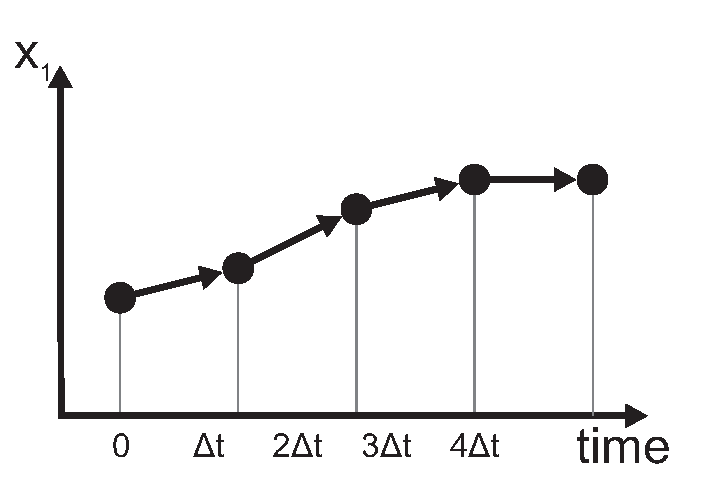
\includegraphics[draft=false,width=0.48\textwidth]{stepper_temporal_evolution.pdf}
\hspace{1ex}
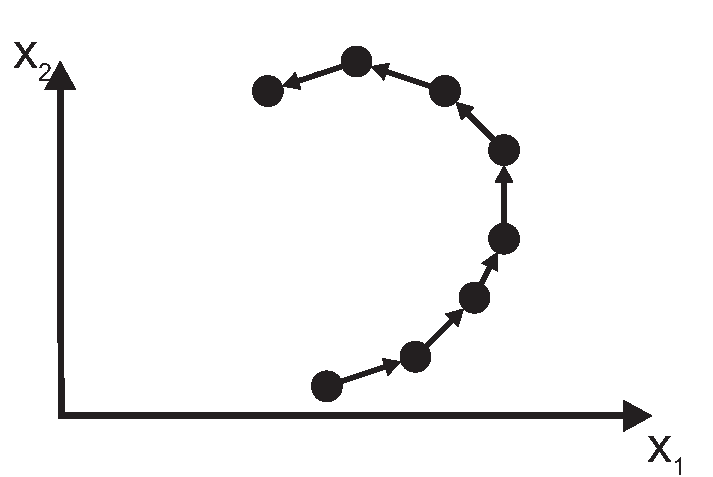
\includegraphics[draft=false,width=0.48\textwidth]{stepper_phase_space.pdf}}
\end{frame}


\rem{
\begin{frame}[fragile]
 \heading{Simulation}

 \vspace{1ex}

 \centerline{Oscillator: $\mu=0 \,\, \text{,} \quad \omega_E = 0 \,\, \text{,} \quad \varepsilon=0$}

 \vspace{1ex}

 \centerline{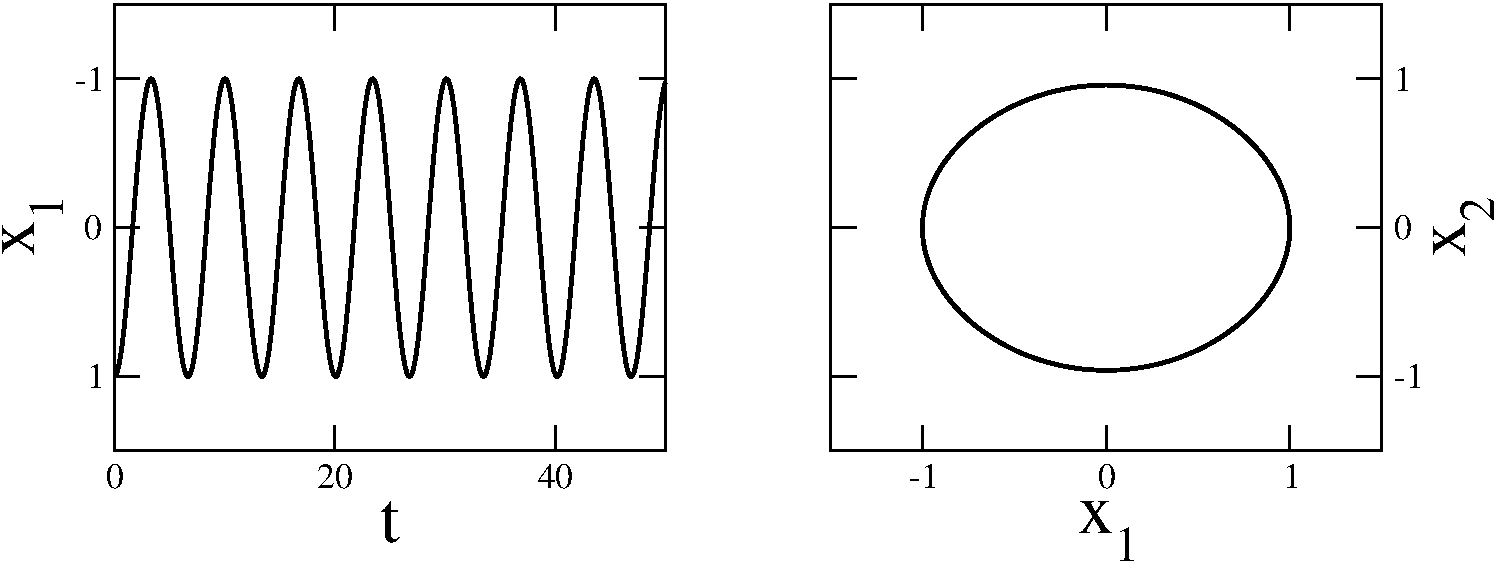
\includegraphics[draft=false,width=0.6\textwidth]{undamped.pdf}}

% \vspace{1ex}
 
\centerline{Damped oscillator: $\mu=0.1 \,\, \text{,} \quad \omega_E = 0 \,\, \text{,} \quad \varepsilon=0$}

 \vspace{1ex}

 \centerline{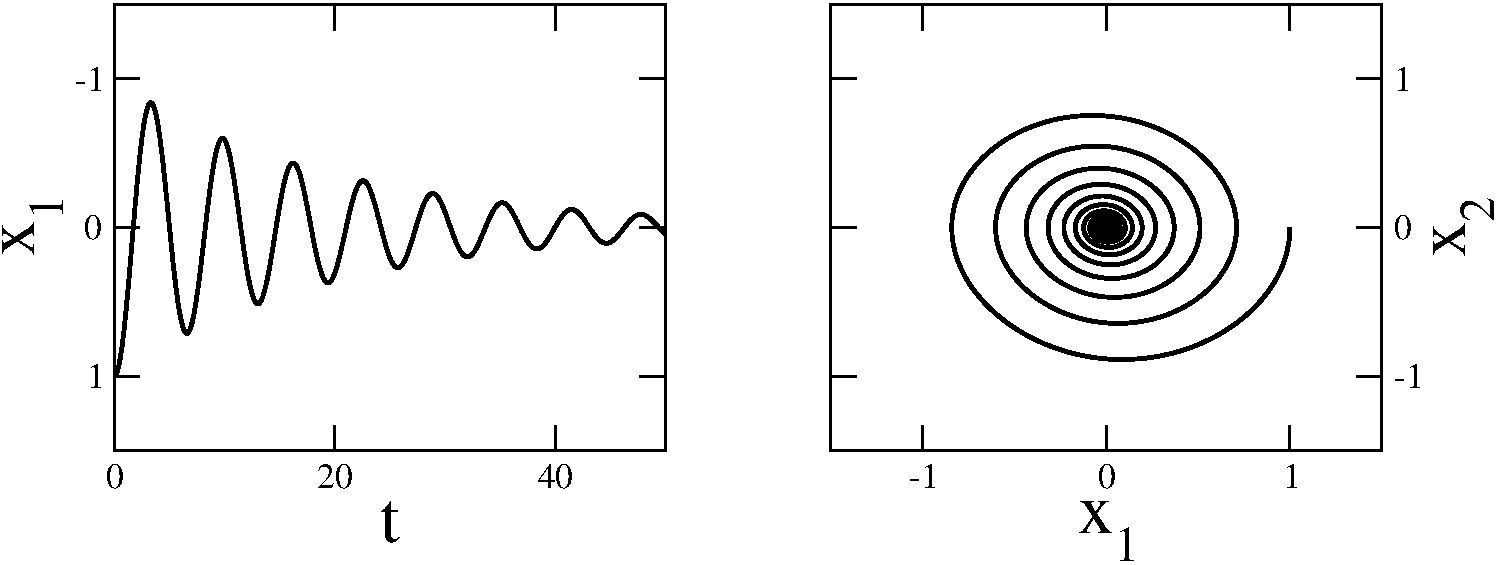
\includegraphics[draft=false,width=0.6\textwidth]{damped.pdf}}

% \vspace{1ex}

 \centerline{Damped, driven oscillator: $\mu=0.1 \,\, \text{,} \quad \omega_E = 1.05 \,\, \text{,} \quad \varepsilon=1.5$}

 \vspace{1ex}

 \centerline{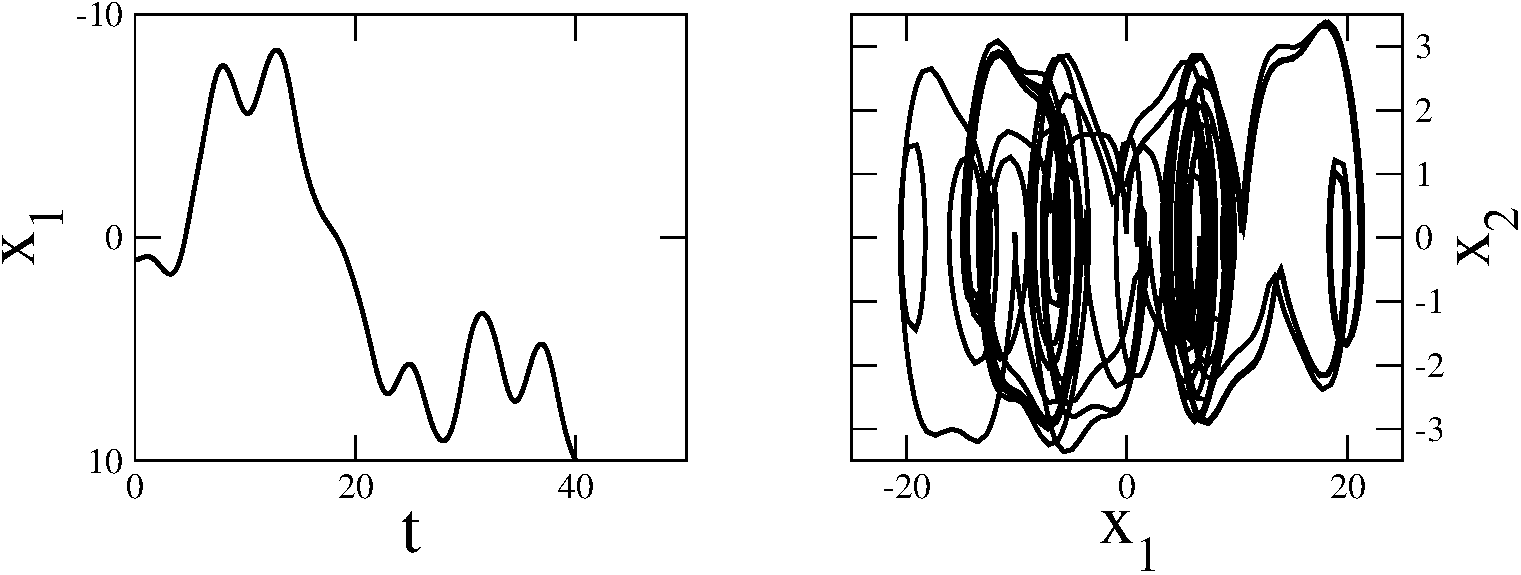
\includegraphics[draft=false,width=0.6\textwidth]{damped_driven.pdf}}


\end{frame}
}





\begin{frame}[fragile]
 \heading{Simulation}

 \vspace{2ex}

\begin{minipage}[t]{0.5\textwidth}
\vspace{0pt}
Oscillator

\vspace{1ex}
$\mu=0 \, \text{,} \,\, \omega_E = 0 \, \text{,} \,\, \varepsilon=0$

\vspace{7ex}
Damped oscillator:

\vspace{1ex}
$\mu=0.1  \, \text{,} \,\, \omega_E = 0  \, \text{,} \,\, \varepsilon=0$

\vspace{7ex}
Damped, driven oscillator:

\vspace{1ex}
$\mu=0.1  \, \text{,} \,\, \omega_E = 1.05  \, \text{,} \,\, \varepsilon=1.5$
\end{minipage}\pause
\begin{minipage}[t]{0.49\textwidth}
\vspace{0pt}
\centerline{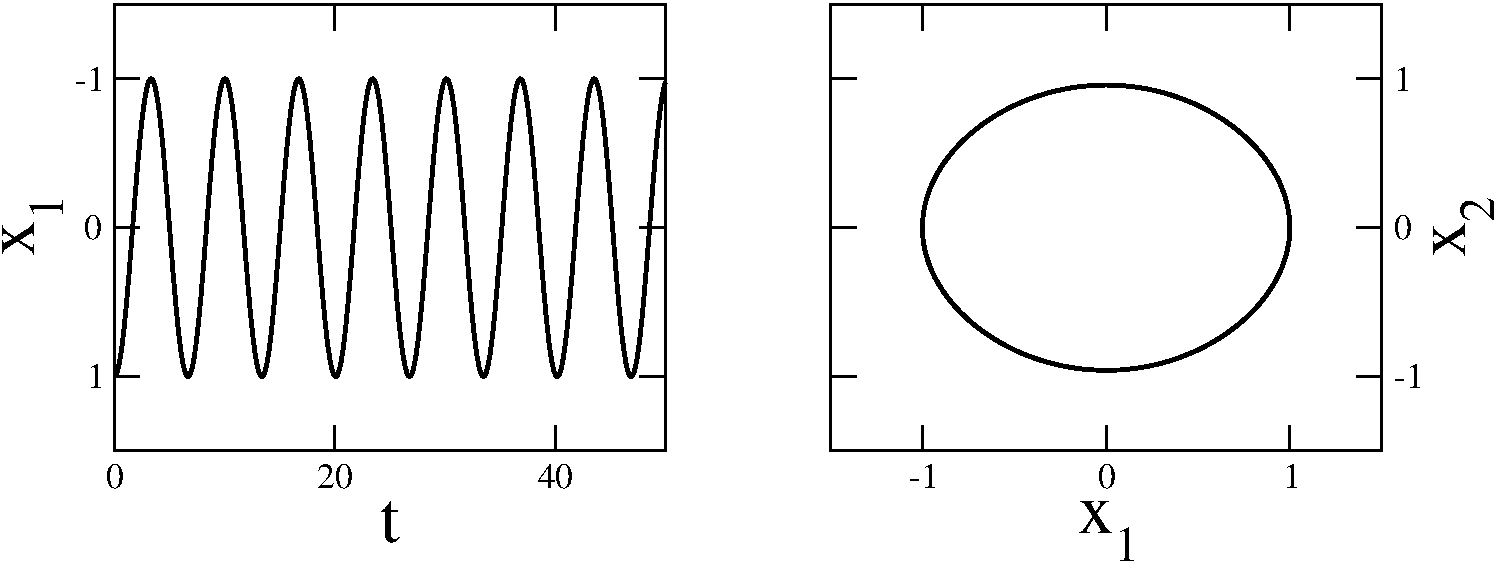
\includegraphics[draft=false,width=1.0\textwidth]{undamped.pdf}}

\vspace{2.5ex}
\centerline{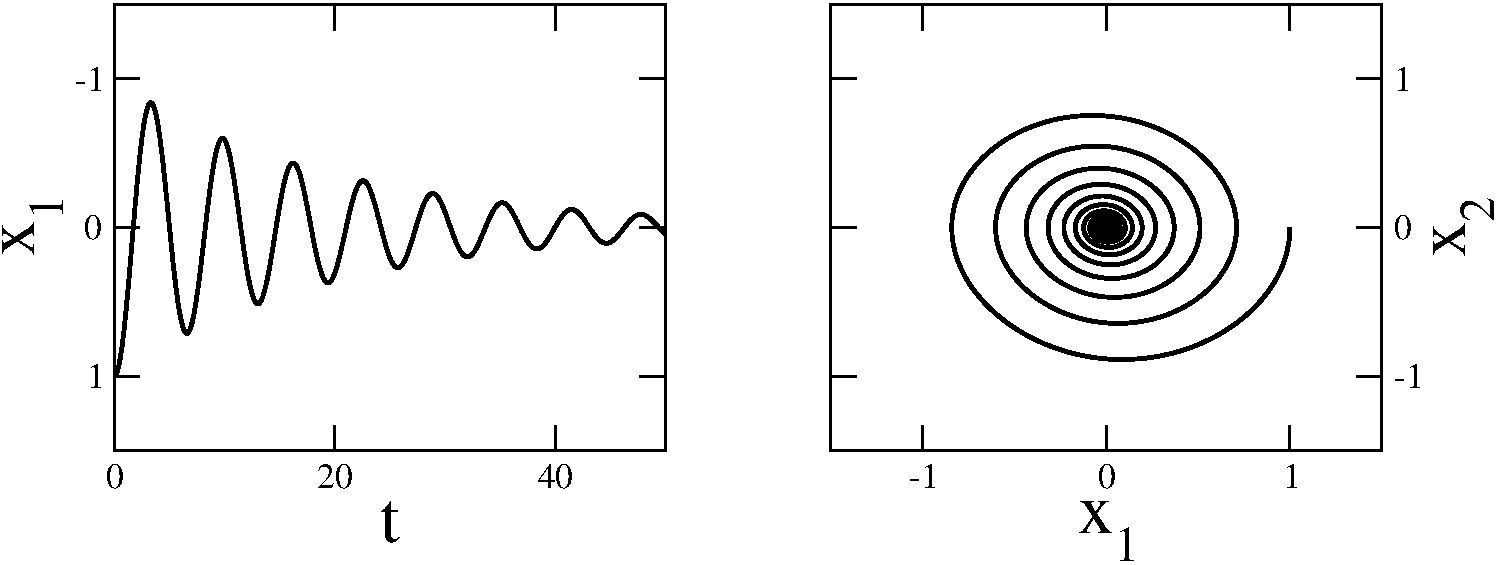
\includegraphics[draft=false,width=1.0\textwidth]{damped.pdf}}

\vspace{2.5ex}
\centerline{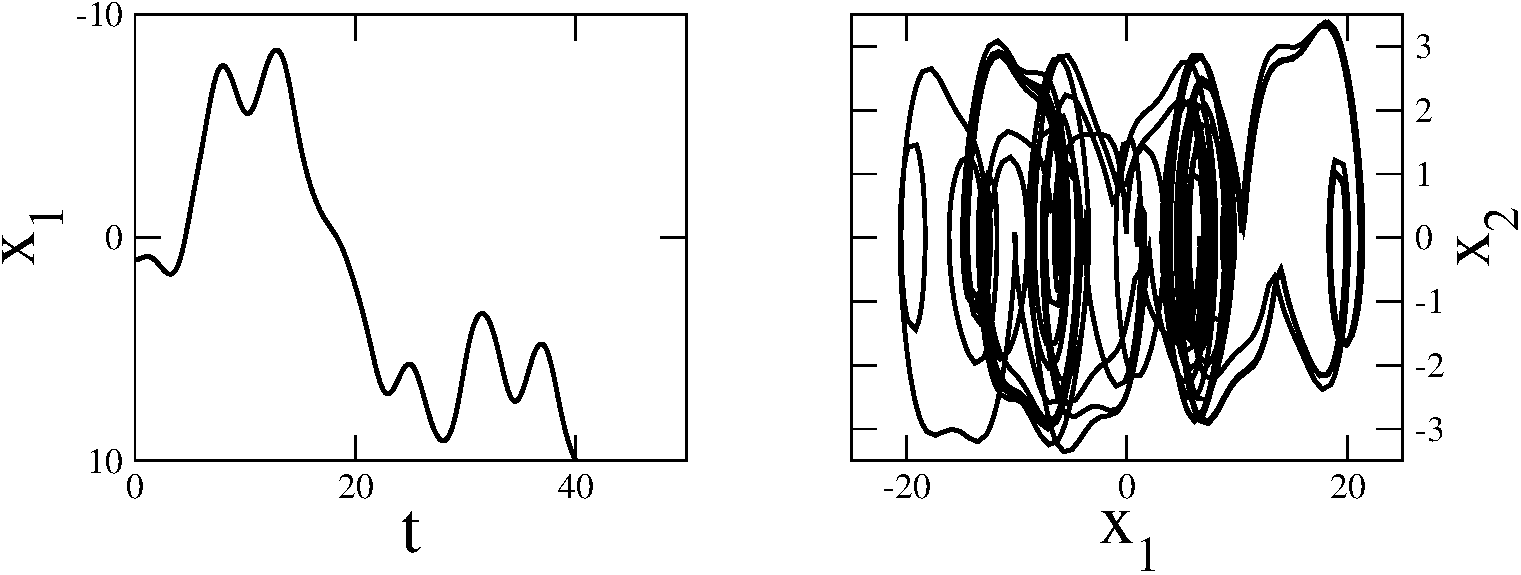
\includegraphics[draft=false,width=1.0\textwidth]{damped_driven.pdf}}
\end{minipage}

\end{frame}







\rem{
\begin{frame}[fragile]

  \heading{Different Steppers}

  \vspace{2ex}

  \begin{lstlisting}
runge_kutta_fehlberg78< state_type > s;
  \end{lstlisting}

  \begin{lstlisting}
runge_kutta_dopri5< state_type > s;
  \end{lstlisting}

  \vspace{2ex}
  Symplectic steppers (for Hamiltonian systems)
  \begin{lstlisting}
symplectic_rkn_sb3a_mclachlan< state_type > s;
  \end{lstlisting}

  \vspace{2ex}
  Implicit steppers (for stiff systems)
  \begin{lstlisting}
rosenbrock4< double > s;
  \end{lstlisting}

  \vspace{2ex}
  {\bf These steppers perform one step with constant step size!}

\end{frame}
}






\begin{frame}
 
 \heading{Controlled steppers -- Step size control}

 \only<1>{
\centerline{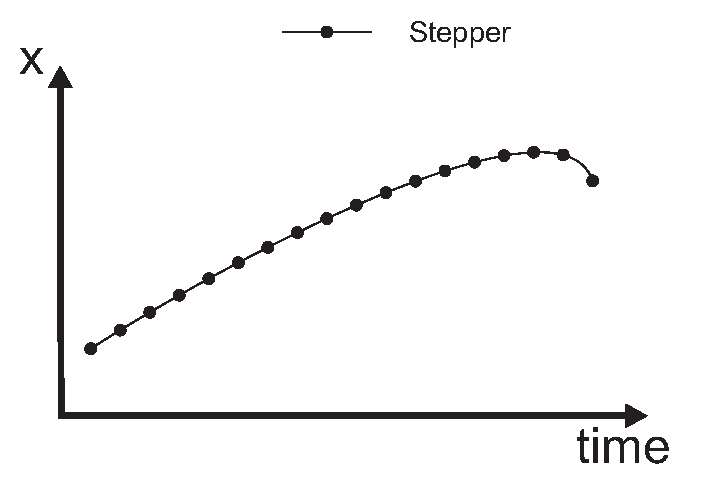
\includegraphics[draft=false,width=0.8\textwidth]{controlled_stepper1.pdf}}
 }
 \only<2>{
\centerline{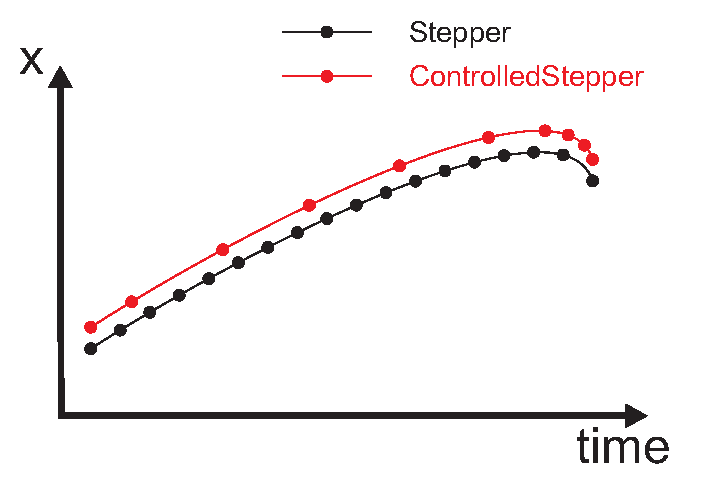
\includegraphics[draft=false,width=0.8\textwidth]{controlled_stepper2.pdf}}
 }


 
\end{frame}



\begin{frame}[fragile]
 
 \heading{Controlled steppers}
 
 \vspace{2ex}

 \begin{lstlisting}
auto s = make_controlled( 1.0e-6 , 1.0e6,
  runge_kutta_fehlberg78<state_type>() );

controlled_step_result res = 
  s.try_step(ode,x,t,dt);
 \end{lstlisting}

 Tries to perform the step and updates $x$, $t$, and $dt$!

 \vspace{4ex}


 It works because Runge-Kutta-Fehlberg has error estimation:

 \begin{lstlisting}
runge_kutta_fehlberg78<state_type> s;
s.do_step(ode,x,t,dt,xerr);
 \end{lstlisting}


\end{frame}


\begin{frame}[fragile]

\heading{Controlled steppers}

\vspace{2ex}

\begin{lstlisting}
auto s = make_controlled(1.0e-6,1.0e6,
  runge_kutta_fehlberg78<state_type>() );
while( t < t_end )
{
  controlled_step_result res;
  do
  { 
    res = s.try_step(ode,x,t,dt);
  }
  while( res != success )
}
\end{lstlisting}

\centerline{Non-trivial time-stepping logic}

\end{frame}


\begin{frame}[fragile]

  \heading{Use integrate functions!}

\vspace{2ex}


\begin{lstlisting}
integrate_adaptive(s,ode,x,t_start,t_end,dt); 
integrate_adaptive(s,ode,x,t_start,t_end,dt,observer);
\end{lstlisting}

Observer: Callable object {\tt obs(x,t)}

\vspace{4ex}
Example (using Boost.Phoenix):
\begin{lstlisting}
integrate_adaptive(s,ode,x,t_start,t_end,dt,
  cout << arg1[0] << " " << arg1[1] << "\n" );
\end{lstlisting}

\vspace{2ex}
More integrate versions:

{\tt integrate\_const}, {\tt integrate\_times}, \dots

\end{frame}



\begin{frame}[fragile]

\heading{Adaptive step size vs. constant step size}

\vspace{2ex}

\begin{lstlisting}
integrate_const(s,ode,x,t,dt,obs);
\end{lstlisting}
\begin{lstlisting}
integrate_adaptive(s,ode,x,t,dt,obs);
\end{lstlisting}

\vspace{2ex}

\centerline{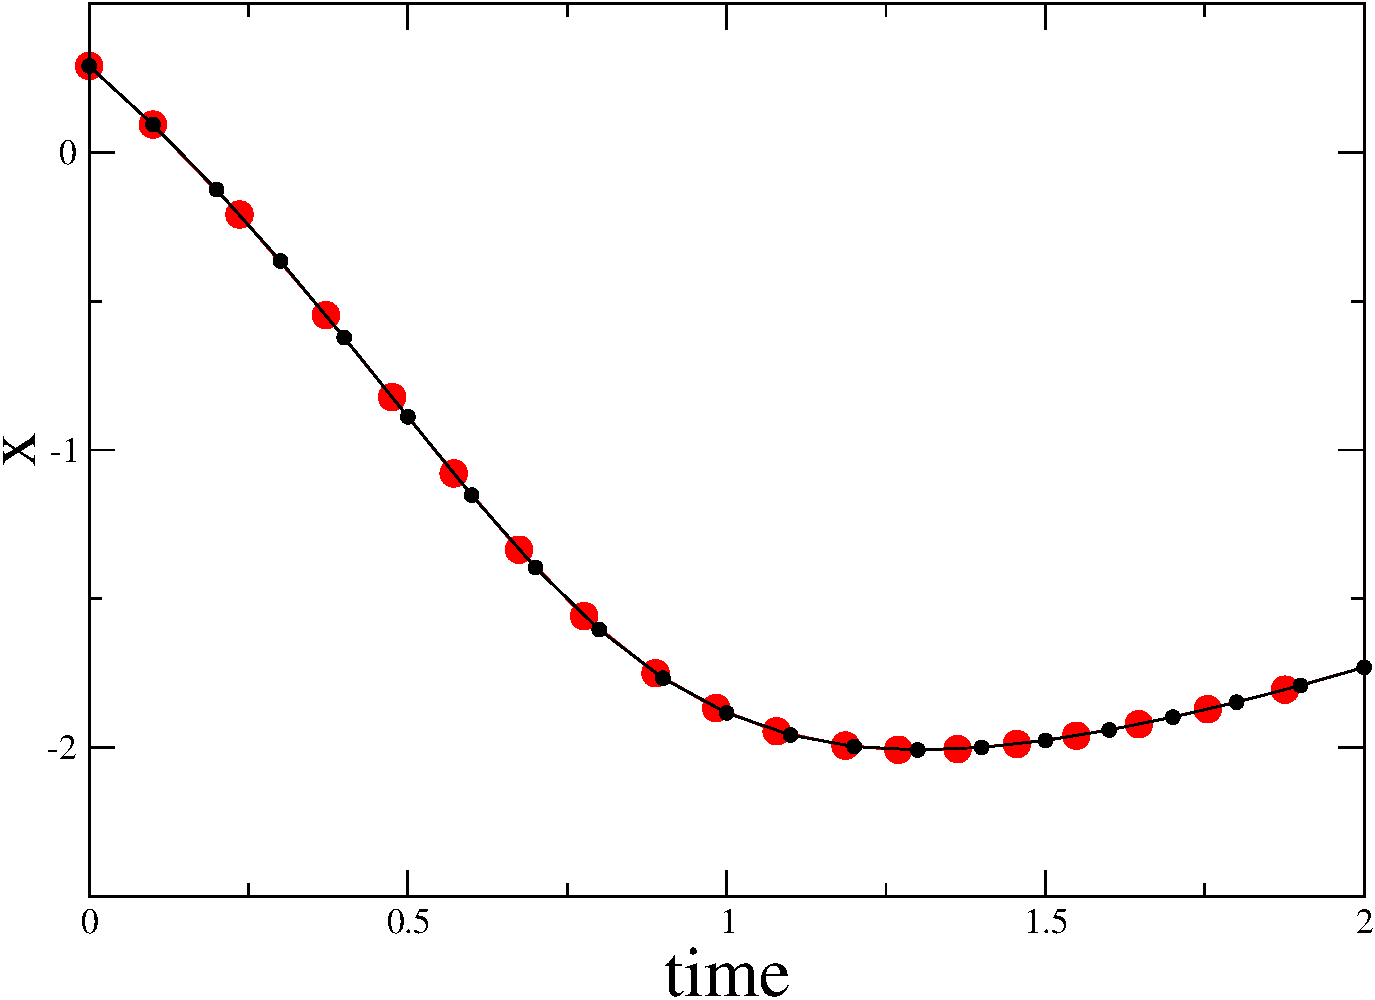
\includegraphics[draft=false,width=0.6\textwidth]{vdp_dense_output.pdf}}

\textbf{Problem:} Equidistant observation with adaptive step size integration?


\end{frame}



\begin{frame}[fragile]

\heading{Dense output stepper}

\vspace{2ex}

\begin{lstlisting}
auto s = make_dense_output( 1.0e-6 , 1.0e-6 ,
    runge_kutta_dopri5< state_type >() );
integrate_const( s , p , x , t , dt );
\end{lstlisting}

Interpolation within integration interval with the same precision as the stepper!

\vspace{2ex}

\centerline{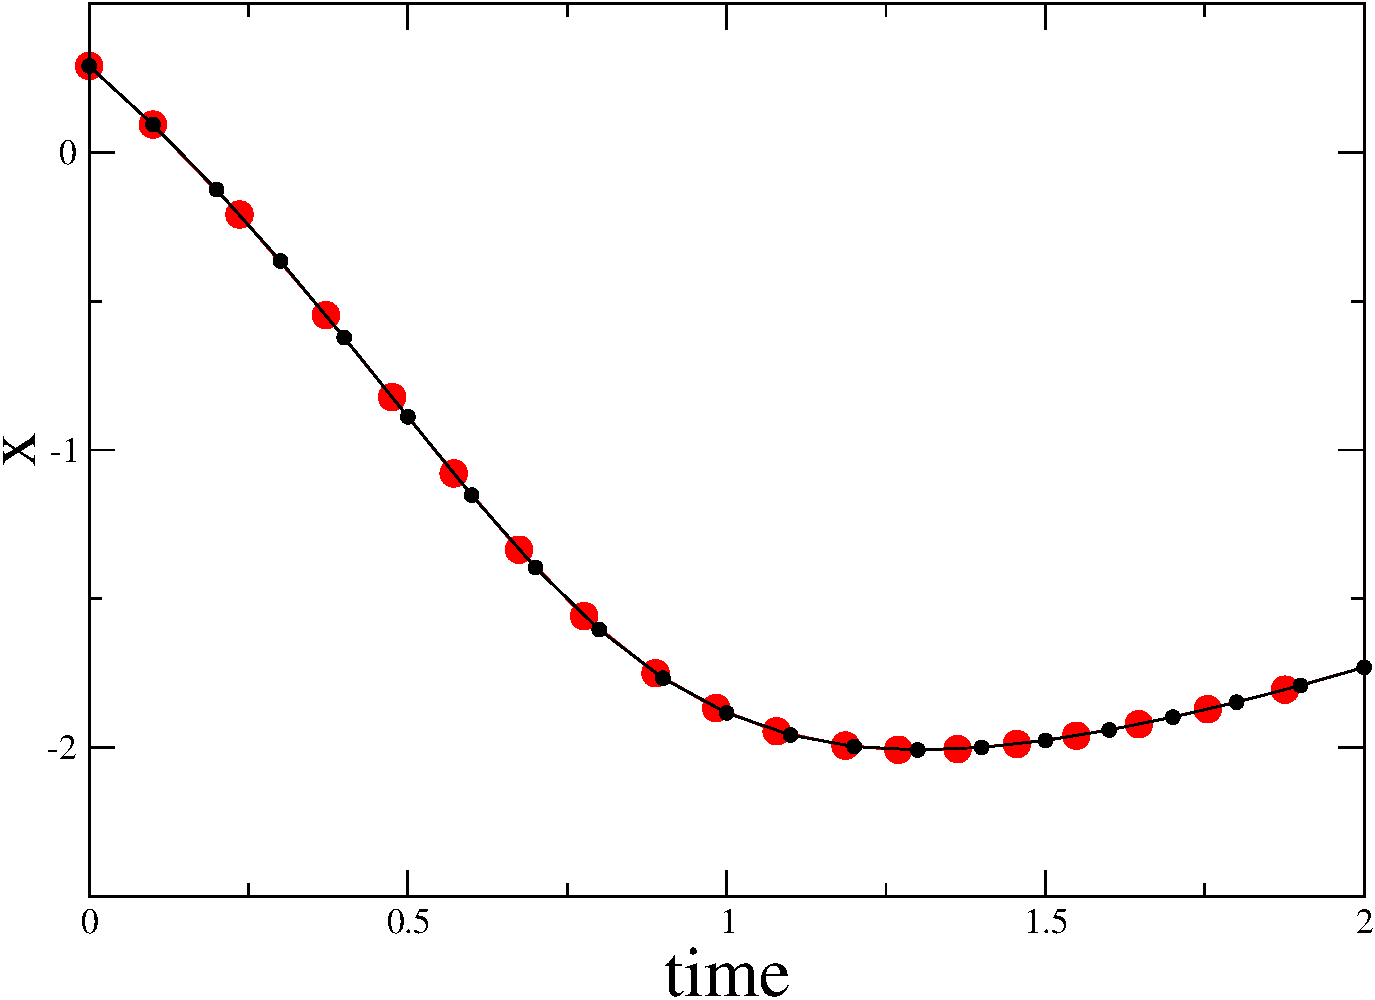
\includegraphics[draft=false,width=0.6\textwidth]{vdp_dense_output.pdf}}

\end{frame}







\begin{frame}
 \heading{More steppers}

 \vspace{2ex}

 {\bf Stepper Concepts}: Stepper, ErrorStepper, ControlledStepper, DenseOutputStepper

 \vspace{2ex}

 {\bf Stepper types}: 
 \begin{itemize}
  \item Implicit -- {\tt implicit\_euler}, {\tt rosenbrock4}
  \item Symplectic -- {\tt symplectic\_rkn\_sb3a\_mclachlan}
  \item Predictor-Corrector -- {\tt adams\_bashforth\_moulton}
  \item Extrapolation -- {\tt bulirsch\_stoer}
  \item Multistep methods -- {\tt adams\_bashforth\_moulton}
 \end{itemize}

 \vspace{2ex}
 Some of them have step-size control and dense-output!

 \vspace{2ex}

 For details see the odeint documentation!

\end{frame}





\begin{frame}
 
 \heading{Small summary}

 \vspace{2ex}
 \begin{itemize}
  \item Very easy example -- nonlinear driven pendulum
  \item Basic features of \odeint
  \item Different steppers -- steppers, error steppers, controlled steppers, dense output steppers
  \item Integrate functions
 \end{itemize}

 \vspace{2ex}

 \pause
 \centerline{\bf Now, let's look at some advanced features!}

\end{frame}



\begin{frame}
 
\heading{Large systems}

\vspace{2ex}

\begin{minipage}{0.48\textwidth} \begin{center}
  Lattice systems

  \vspace{3ex}

  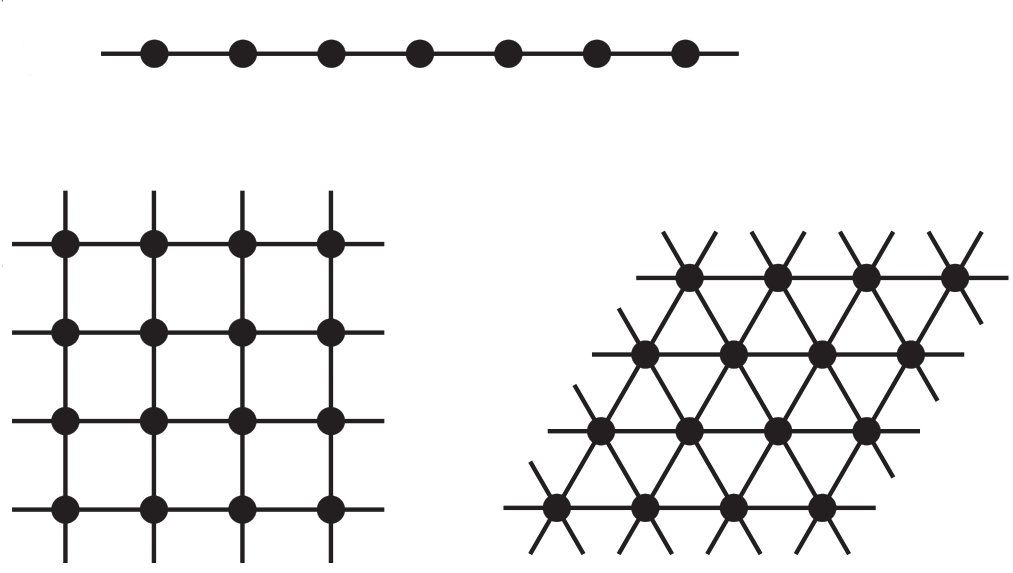
\includegraphics[draft=false,width=0.8\textwidth]{lattices.jpg}
\end{center} \end{minipage}
\pause
\begin{minipage}{0.48\textwidth} \begin{center}
  Discretiztations of PDEs

  \vspace{0.5ex}
  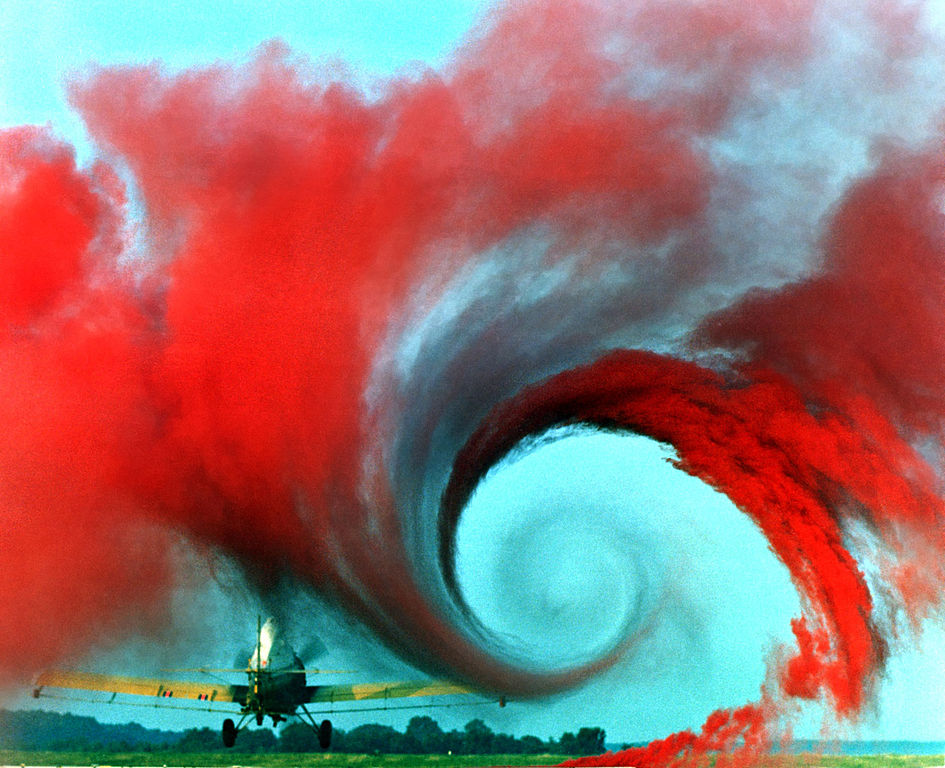
\includegraphics[draft=false,width=0.7\textwidth]{turbulence.jpg}
\end{center} \end{minipage}

\pause
\vspace{2ex}

\begin{minipage}{0.48\textwidth}\begin{center}
  ODEs on graphs

  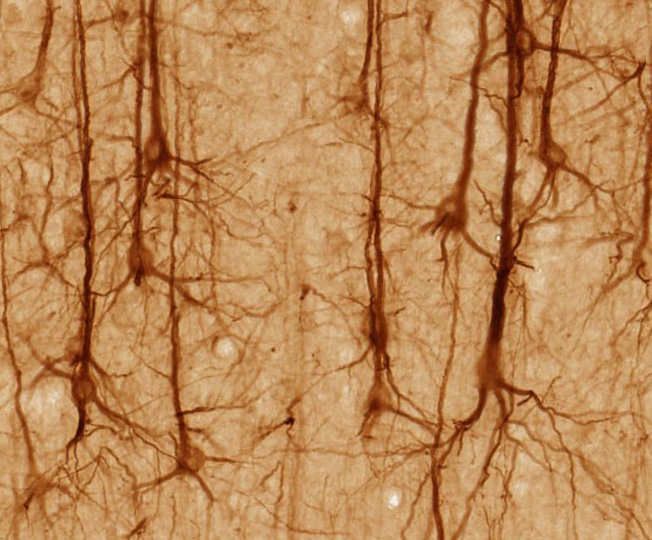
\includegraphics[draft=false,width=0.7\textwidth]{neuron.jpg}
 \end{center}\end{minipage}\pause
\begin{minipage}{0.48\textwidth}\begin{center}
  Parameter studies
 
  \vspace{0.5ex}
  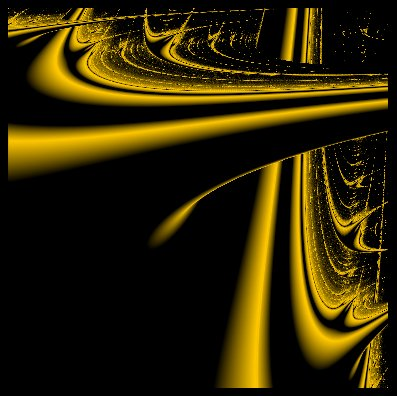
\includegraphics[draft=false,width=0.59\textwidth]{lyap.jpg}
 \end{center} \end{minipage}



\end{frame}







\rem{
\begin{frame}[fragile]
 \heading{Coupled phase oscillators}

 \vspace{2ex}

 \begin{columns}[T]
  \begin{column}{0.35\textwidth}
   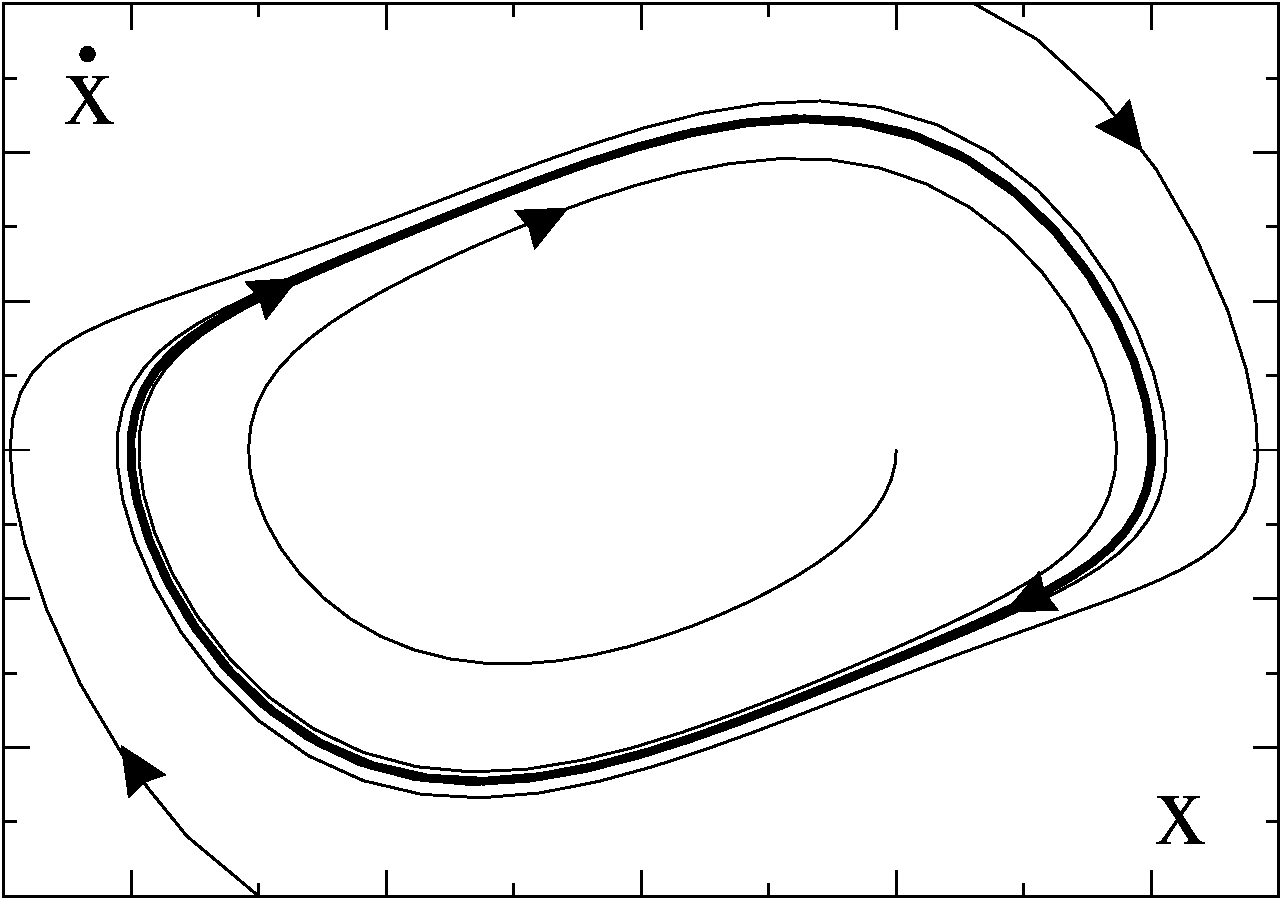
\includegraphics[draft=false,width=1.0\textwidth]{vdp.pdf}  
  \end{column}
  \begin{column}{0.63\textwidth}
 Any oscillator can be described by one variable -- its phase!

 \vspace{2ex}

 Trivial dynamic: $\dot{\varphi}=\omega$

  \end{column}
 \end{columns}

 \pause


 \vspace{2ex}

 Interesting behaviour occurs if oscillators are coupled.

 \begin{itemize}
  \item Synchronization, oscillation death, phase chaos, pattern formation, \dots
 \end{itemize}

 Applications: Neurosciences, Heart dynamics, social systems

 \vspace{2ex}

 Any weakly coupled oscillator system

 \vspace{1ex}

 \centerline{$\dot{\varphi}_k = \omega_k + q( \varphi_{k+1} , \varphi_k ) + q( \varphi_k , \varphi_{k-1} )$}

   
 
\end{frame}
}



\begin{frame}[fragile]
 
 \heading{Phase compacton lattice}

 \vspace{2ex}

 $$\dot{\varphi}_k = \cos \varphi_{k+1} - \cos \varphi_{k-1}$$

 \vspace{2ex}

 State space contains $N$ variables

 \begin{lstlisting}
typedef std::vector<double> state_type;
 \end{lstlisting}

 \vspace{2ex}

 \centerline{Simulation}

\end{frame}

\begin{frame}[fragile]

 \heading{Phase compacton lattice -- Space-time plots}

 \vspace{2ex}

\centerline{\begin{sideways}\hspace{0ex}spatial index\end{sideways} 
\includegraphics[draft=false,width=0.9\textwidth]{transition_chaos_1.jpg}}

\centerline{time}


\vspace{4ex}
\centerline{\begin{sideways}\hspace{0ex}spatial index\end{sideways} 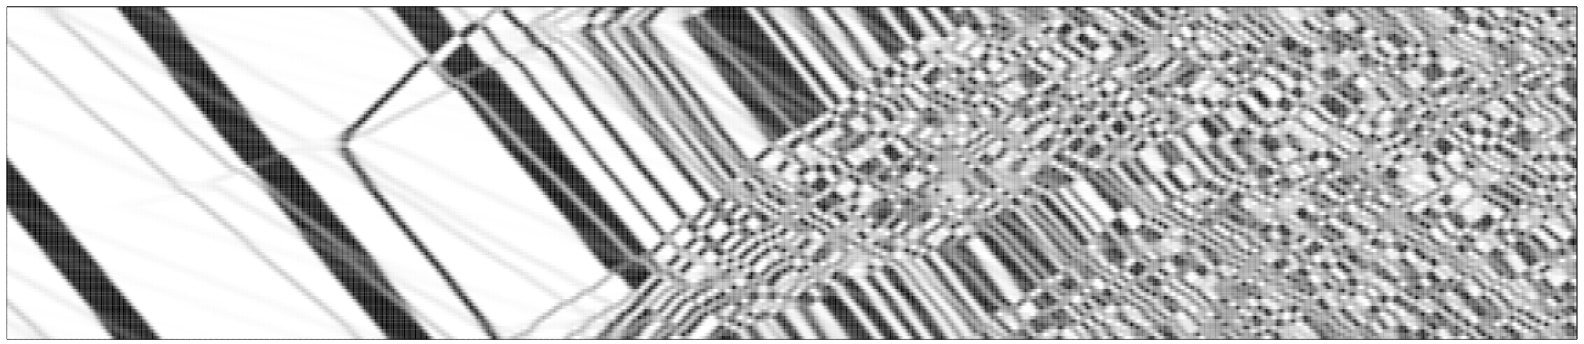
\includegraphics[draft=false,width=0.9\textwidth]{transition_chaos_2.jpg}}

\centerline{time}
 
\end{frame}








\rem{
\begin{frame}[fragile]

 \heading{Ensemble of phase oscillators -- SKIP}

 \vspace{2ex}

$$\dot{\varphi}_k = \omega_k + \sum\limits_l \sin( \varphi_l - \varphi_k )$$

{\bf Synchronization} -- all oscillator oscillates with the same frequency

 \vspace{2ex}

Synchronized state $\varphi_k = \omega_S t + \varphi_{0,k} $

\end{frame}





\begin{frame}[fragile]

\heading{Ensemble of phase oscillators -- SKIP}

\begin{lstlisting}
typedef std::vector<double> state_type;

struct ensemble
{
    state_type m_omega,m_eps;

    ensemble(size_t n,double eps)
    : m_omega(n,0.0),m_eps(eps)
    {
        create_frequencies();
    }

    void create_frequencies() { ... }

    void operator()(const state_type &x,state_type &dxdt,double t) const
    {
         ...
    }
};
\end{lstlisting}

The ODE has now many parameters, use boost::ref

Vielleicht koennen diese beiden Folien weg

\end{frame}
}


\begin{frame}[fragile]

\heading{Solving ODEs with CUDA using Thrust}

\vspace{4ex}
\begin{quotation}
``Thrust is a parallel algorithms library which resembles the C++ Standard Template Library (STL). Thrust's high-level interface greatly enhances developer productivity while enabling performance portability between GPUs and multicore CPUs. Interoperability with established technologies (such as CUDA, TBB and OpenMP) facilitates integration with existing software. Develop high-performance applications rapidly with Thrust!''
\end{quotation}

\vspace{2ex}

\centerline{
\includegraphics[draft=false,width=0.3\textwidth]{thrust_logo.png}}
 

\end{frame}


\begin{frame}[fragile]
 
\heading{Solving ODEs with CUDA using thrust}

\vspace{2ex}
Applications and use cases for GPUs:

\begin{itemize}
 \item Large systems, discretizations of PDEs, lattice systems, granular systems, etc.
 \item Parameter studies, solve many ODEs in parallel with different parameters
 \item Initial value studies, solve the same ODE with many different initial conditions in parallel
\end{itemize}


\end{frame}



\begin{frame}[fragile]
 
\heading{Nonlinear pendulum -- Deterministic chaos}

 $$
  \dot{x} = y \quad \quad \dot{y} = - \sin(x) - \mu y + \varepsilon \sin \omega_E t 
 $$

\vspace{2ex}
Perturbations grow exponentially fast -- Butterfly effect

\vspace{2ex}

\centerline{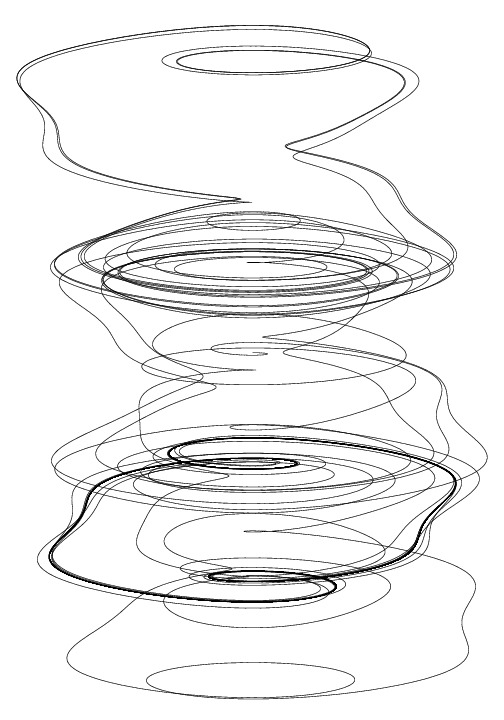
\includegraphics[draft=false,angle=270,width=0.6\textwidth]{pendulum2.jpg}}

\end{frame}



\begin{frame}[fragile]
 
  \heading{Nonlinear pendulum -- Parameter study}


$$
  \dot{x} = y \quad \quad \dot{y} = - \sin(x) - \mu y + \varepsilon \sin \omega_E t 
 $$


Does one observe chaos over the whole parameter range?

\vspace{2ex}

Lyapunov exponents:
\begin{itemize}
 \item Measure of chaos
 \item Growth rate of perturbations
\end{itemize}

\vspace{2ex}
Vary $\varepsilon$ from $0$ to $5.0$ and $\omega_E$ from $0.5$ to $1.5$ and calculate the Lyapunov exponents!

\vspace{2ex}
\centerline{\bf Use CUDA and Thrust!}

\end{frame}





\rem{

\begin{frame}[fragile]
 
\heading{Lorenz system -- Deterministic chaos}

 $$
  \dot{x} = \sigma ( y - x ) \quad \quad \dot{y} = R x - y - x z \quad \quad \dot{z} = -b z + x y
 $$

Standard parameters $\sigma=10$, $R=28$, $b=8/3$

\vspace{2ex}
Perturbations grow exponentially fast -- Butterfly effect

\vspace{4ex}

\centerline{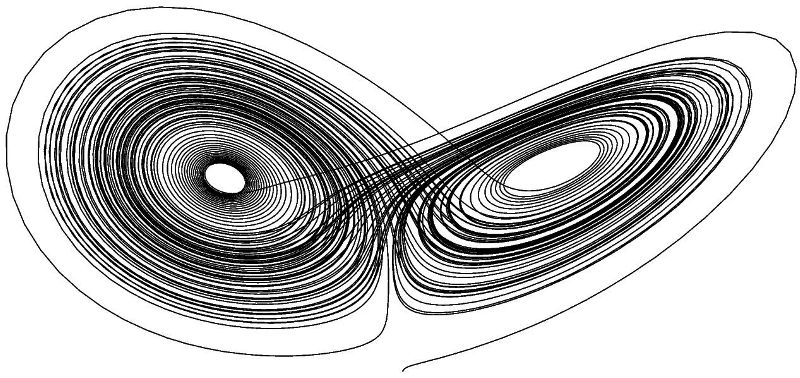
\includegraphics[draft=false,width=0.8\textwidth]{lorenz.jpg}}

\end{frame}



\begin{frame}[fragile]
 
  \heading{Lorenz system -- Parameter study}


 $$
  \dot{x} = \sigma ( y - x ) \quad \quad \dot{y} = R x - y - x z \quad \quad \dot{z} = -b z + x y
 $$


Does one observe chaos over the whole parameter range?

\vspace{2ex}

Lyapunov exponents:
\begin{itemize}
 \item Measure of chaos
 \item Growth rate of perturbations
\end{itemize}

\vspace{2ex}
Vary $R$ from $0$ to $50$ and calculate the Lyapunov exponents!

\vspace{2ex}
\centerline{\bf Use CUDA and Thrust!}

\end{frame}

}



\begin{frame}[fragile]

 \heading{Intermezzo: Algebras and operations}

 \vspace{2ex}

Euler method

$$\text{for all i :}  \quad \quad x_i(t+\Delta t) = x_i(t) + \Delta t \cdot f_i(x)$$

\vspace{2ex}

\begin{lstlisting}
typedef euler< state_type ,
   value_type , deriv_type , time_type,
   algebra , operations , resizer > stepper; 
\end{lstlisting}


\begin{itemize}
\item Algebras perform the iteration over $i$.
\item Operations perform the elementary addition.
\end{itemize}


\end{frame}

\begin{frame}[fragile]

 \heading{Intermezzo: Algebras and operations}

\begin{lstlisting}
typedef euler< state_type ,
   value_type , deriv_type , time_type,
   algebra , operations , resizer > stepper; 
\end{lstlisting}

Default template parameters:

\begin{itemize}
 \item {\tt range\_algebra} -- Boost.Ranges
 \item {\tt default\_operations}
\end{itemize}

\vspace{2ex}
For Thrust:

\begin{itemize}
 \item {\tt thrust\_algebra}
 \item {\tt thrust\_operations}
 \item {\tt thrust::device\_vector}
\end{itemize}

 
\end{frame}



\begin{frame}[fragile]

 \heading{Calculate an ensemble of pendulums}

 \begin{lstlisting}[basicstyle=\scriptsize\ttfamily]
typedef thrust::device_vector<double> state_type;
typedef runge_kutta4<state_type,double,state_type,double,
   thrust_algebra,thrust_operations> stepper; 

state_type x( 2*N );
// initialize x
integrate_const( stepper() , pendulum_ensemble() ,
   x , 0.0 , 1000.0 , dt );
 \end{lstlisting}

\vspace{2ex}

\centerline{Memory layout:}

\vspace{1ex}

\centerline{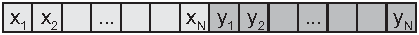
\includegraphics[draft=false,width=0.7\textwidth]{memory_layout2.pdf}}

\vspace{6ex}

\centerline{Everything seems easy!}
\vspace{2ex}
\centerline{{\bf But} how does {\tt pendulum\_ensemble} look like?}
 

\end{frame}




\begin{frame}[fragile]

 \heading{Ensemble of nonlinear pendulums}

 \begin{lstlisting}[basicstyle=\scriptsize\ttfamily]
struct pendulum_ensemble {
  size_t N;
  state_type eps , omega;

  template< class State , class Deriv >
  void operator()(
    const State &x , Deriv &dxdt , value_type t ) const {
  
    thrust::for_each(
      thrust::make_zip_iterator( thrust::make_tuple(
        x.begin() , x.begin()+N , 
        eps.begin() , omega.begin() , 
        dxdt.begin(), dxdt.begin()+N 
      ) ) ,
      thrust::make_zip_iterator( thrust::make_tuple(
        x.begin()+N , x.begin()+2*N 
        eps.end() , omega.end() ,
        dxdt.begin()+N,dxdt.begin()+2*N
      ) ) ,
      pendulum_functor(t) );
  }

  // ...
};
 \end{lstlisting}


\end{frame}


\begin{frame}[fragile]

 \heading{Ensemble of nonlinear pendulums}

 \begin{lstlisting}[basicstyle=\scriptsize\ttfamily]
struct pendulum_ensemble
{
  // ...

  struct pendulum_functor
  {
    double time;
    pendulum_functor( double _time ) : time(_time) { }
    
    template< class T > __host__ __device__
    void operator()( T t ) const
    {
      value_type x = thrust::get< 0 >( t );
      value_type y = thrust::get< 1 >( t );
      value_type eps = thrust::get< 2 >( t );
      value_type omega = thrust::get< 3 >( t );
      thrust::get< 4 >( t ) = x
      thrust::get< 5 >( t ) = -x - mu*y
            + eps * sin( omega * time );
    }
  };
};
 \end{lstlisting}


\end{frame}


\rem{

\begin{frame}[fragile]

 \heading{Nonlinear pendulum parameter study -- Results}

 \vspace{4ex}

\centerline{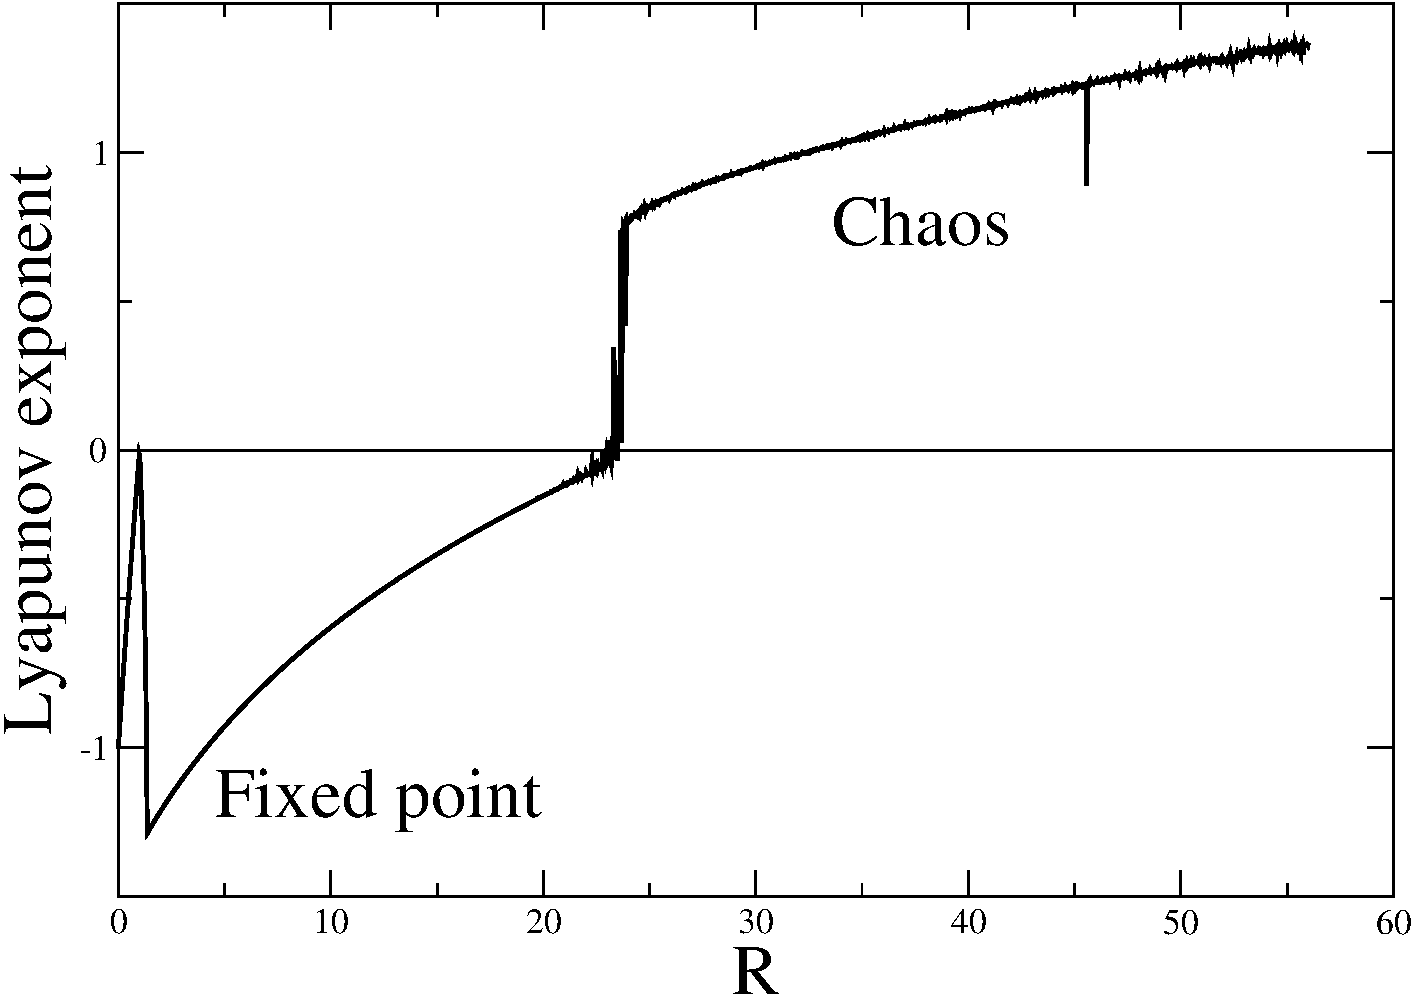
\includegraphics[draft=false,width=0.8\textwidth]{lyap_lorenz.pdf}}

\end{frame}

}








\rem{

\begin{frame}[fragile]

 \heading{Calculate an ensemble of Lorenz systems}

 \begin{lstlisting}[basicstyle=\scriptsize\ttfamily]
typedef thrust::device_vector<double> state_type;
typedef runge_kutta4<state_type,double,state_type,double,
   thrust_algebra,thrust_operations> stepper; 

state_type x( 3*N );
// initialize x
integrate_const( stepper() , lorenz_ensemble() ,
   x , 0.0 , 1000.0 , dt );
 \end{lstlisting}

\vspace{2ex}

\centerline{Memory layout:}

\vspace{1ex}

\centerline{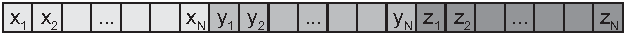
\includegraphics[draft=false,width=0.9\textwidth]{memory_layout.pdf}}

\vspace{6ex}

\centerline{Everything seems easy!}
\vspace{2ex}
\centerline{{\bf But} how does {\tt lorenz\_ensemble} look like?}
 

\end{frame}




\begin{frame}[fragile]

 \heading{Ensemble of Lorenz systems}

 \begin{lstlisting}[basicstyle=\scriptsize\ttfamily]
struct lorenz_ensemble {
  size_t N;
  state_type R;

  template< class State , class Deriv >
  void operator()(
    const State &x , Deriv &dxdt , value_type t ) const {
  
    thrust::for_each(
      thrust::make_zip_iterator( thrust::make_tuple(
        x.begin() , x.begin()+N , x.begin()+2*N ,
        R.begin() ,
        dxdt.begin(), dxdt.begin()+N, dxdt.begin()+2*N
      ) ) ,
      thrust::make_zip_iterator( thrust::make_tuple(
        x.begin()+N , x.begin()+2*N , x.begin()+3*N ,
        R.end() ,
        dxdt.begin()+N,dxdt.begin()+2*N,dxdt.begin()+3*N
      ) ) ,
      lorenz_functor() );
  }

  // ...
};
 \end{lstlisting}


\end{frame}


\begin{frame}[fragile]

 \heading{Ensemble of Lorenz systems}

 \begin{lstlisting}[basicstyle=\scriptsize\ttfamily]
struct lorenz_ensemble
{
  // ...

  struct lorenz_functor
  {
    template< class T > __host__ __device__
    void operator()( T t ) const
    {
      value_type R = thrust::get< 3 >( t );
      value_type x = thrust::get< 0 >( t );
      value_type y = thrust::get< 1 >( t );
      value_type z = thrust::get< 2 >( t );
      thrust::get< 4 >( t ) = sigma * ( y - x );
      thrust::get< 5 >( t ) = R * x - y - x * z;
      thrust::get< 6 >( t ) = -b * z + x * y ;
    }
  };
};
 \end{lstlisting}


\end{frame}




\begin{frame}[fragile]

 \heading{Lorenz system parameter study -- Results}

 \vspace{4ex}

\centerline{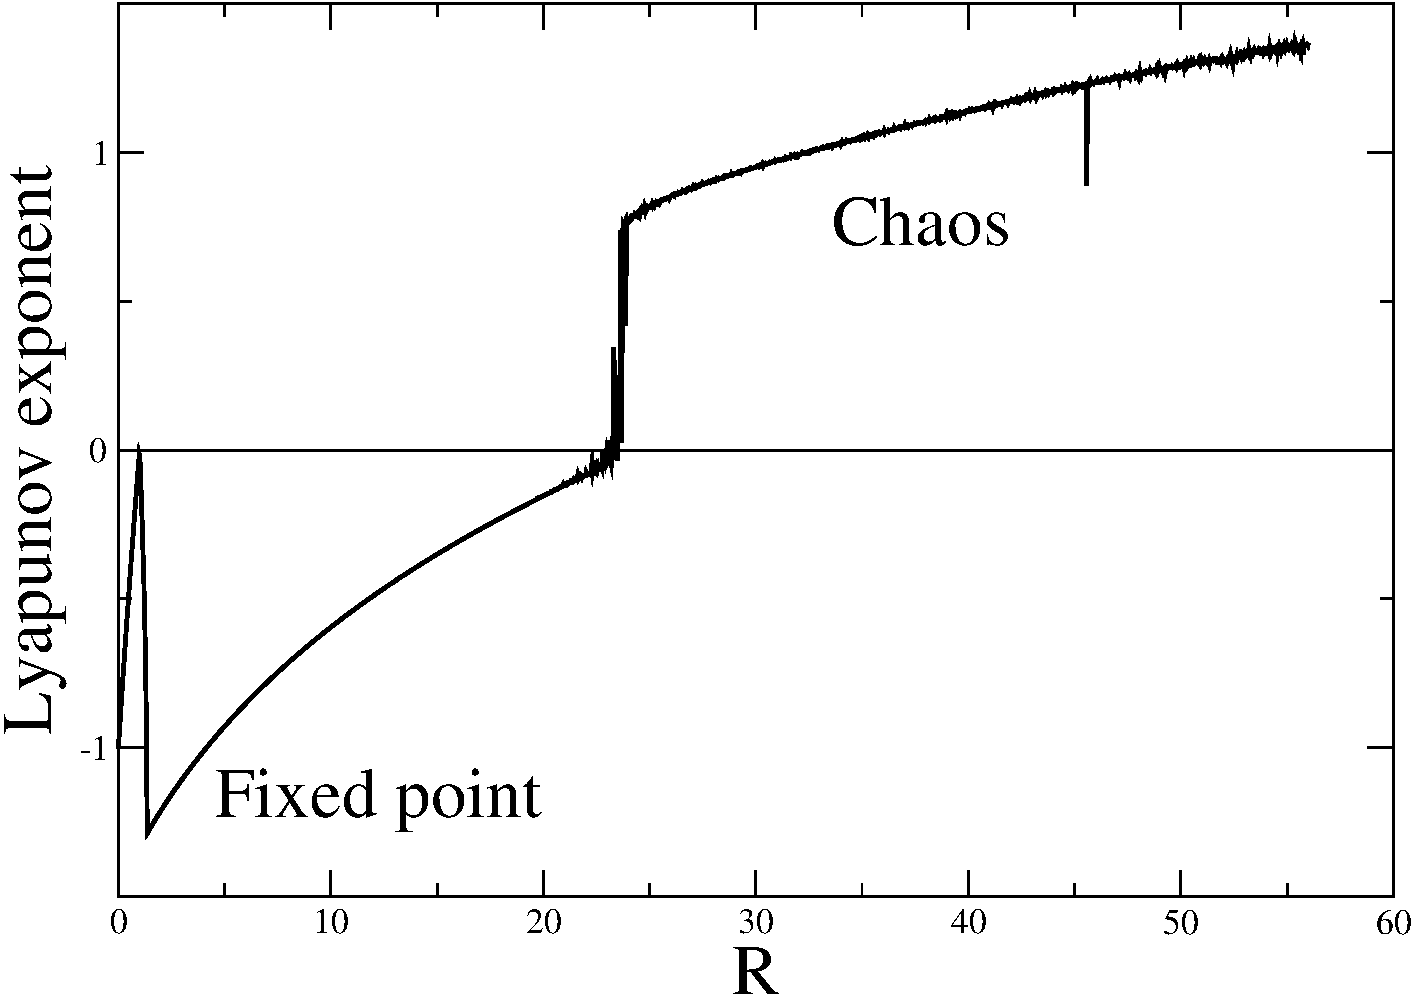
\includegraphics[draft=false,width=0.8\textwidth]{lyap_lorenz.pdf}}

\end{frame}

}









\begin{frame}
 \heading{Advanced features - continued}

\end{frame}


\begin{frame}[fragile]
 \heading{Reference wrapper {\tt std::ref}, {\tt boost::ref}}

\vspace{2ex}

 The ODE and the observers are always passed by value

 \begin{lstlisting}
integrate_const{s,ode,x,0.0,1.0,dt,obs);
s.do_step(ode,x,t,dt);
 \end{lstlisting}

\pause

\vspace{2ex}
Use {\tt std::ref} or {\tt boost::ref} to pass by reference
 \begin{lstlisting}
integrate_const{s,std::ref(ode),x,0.0,1.0,dt,
  std::ref(obs));
 \end{lstlisting}

\end{frame}



\begin{frame}[fragile]
 \heading{Using Boost.Range}

 \vspace{2ex}
 Use Boost.Range to integrate separate parts of the overall state

 \vspace{2ex}
 Example: Lyapunov exponents for the Lorenz system

 \vspace{2ex}

 \centerline{\bf Complete ODE = Lorenz system + Perturbation}


 \begin{itemize}
  \item Calculate transients by solving only the Lorenz system (initialize $x,y,z$)
  \item Solve whole system (state + perturbations)
 \end{itemize}

\vspace{2ex}

 \begin{lstlisting}
std::vector<double> x(6,0.0);
integrate(s,lorenz,
  make_pair(x.begin(),x.begin()+3),
  0.0,10.0,dt);
integrate(s,lorenz_pert,x,10.0,1000.0,dt);
 \end{lstlisting}



\end{frame}



\begin{frame}[fragile]
 \heading{ODEs with complex numbers}

 \vspace{2ex}

 Discrete Nonlinear Schr\"odinger equation
$$
  \ii \dot{\Psi}_k = \varepsilon_k \Psi_k + V( \Psi_{k+1}+\Psi_{k-1}) - \gamma |\Psi_k|^2 \Psi_k
  \quad \quad \text{,} \quad \Psi_k \in \mathbb{C}
$$
 

 \begin{lstlisting}[basicstyle=\scriptsize\ttfamily]
typedef std::vector<std::complex<double> > state_type;

struct dnls
{
  std::vector<double> eps;
  void operator()(const state_type &x, state_type &dxdt,
    double t) const
  {
    // ...
  }
};

runge_kutta_fehlberg78< state_type > stepper;
 \end{lstlisting}

\end{frame}

\begin{frame}[fragile]
 \heading{Matrices as state types}

 \vspace{1ex}
 \begin{columns}[T]
  \begin{column}{0.35\textwidth}
   \centerline{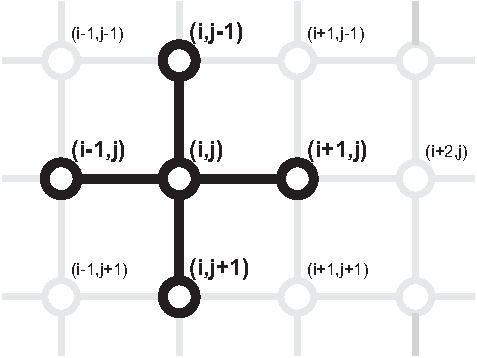
\includegraphics[draft=false,width=0.9\textwidth]{2dlattice.pdf}}
  \end{column}
  \begin{column}{0.58\textwidth}
Example: 

\vspace{1ex}
Two-dimensional phase lattice
\begin{align*}
\dot{\varphi}_{i,j} = &
  q(\varphi_{i+1,j},\varphi_{i,j}) 
 + q(\varphi_{i-1,j},\varphi_{i,j}) \\
 + & q(\varphi_{i,j+1},\varphi_{i,j}) 
 + q(\varphi_{i,j-1},\varphi_{i,j})
 \end{align*}
  \end{column}
 \end{columns}

\vspace{1ex}

\begin{lstlisting}[basicstyle=\scriptsize\ttfamily]
typedef ublas::matrix<double> state_type1;
typedef mtl::dense2D<double> state_type2;

runge_kutta_fehlberg78< state_type1 , double ,
  state_type1 , double , vector_space_algebra > stepper1;
\end{lstlisting}

\pause
\vspace{1ex}


\centerline{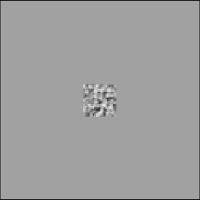
\includegraphics[draft=false,width=0.27\textwidth]{phase_lattice_2d_0000.jpg} \hspace{2ex}
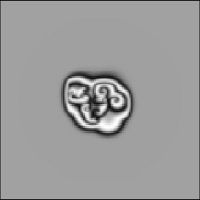
\includegraphics[draft=false,width=0.27\textwidth]{phase_lattice_2d_0100.jpg} \hspace{2ex}
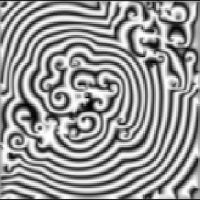
\includegraphics[draft=false,width=0.27\textwidth]{phase_lattice_2d_1000.jpg}}
\end{frame}

\begin{frame}[fragile]
 \heading{Compile-time sequences and Boost.Units}

 $$
 \left( \begin{array}{c} \dot{x} \\ \dot{v} \end{array} \right) 
= \left( \begin{array}{l} v \\ f(x,v) \end{array} \right)
$$
 \begin{itemize}
  \item $x$ -- length, dimension $m$
  \item $v$ -- velocity, dimension $m s^{-1}$
  \item $a$ -- acceleration, dimension $m s^{-2}$
 \end{itemize}

 \begin{lstlisting}[basicstyle=\tiny\ttfamily]
typedef units::quantity< si::time , double > time_type;
typedef units::quantity< si::length , double > length_type;
typedef units::quantity< si::velocity , double > velocity_type;
typedef units::quantity< si::acceleration , double > acceleration_type;

typedef fusion::vector< length_type , velocity_type > state_type;
typedef fusion::vector< velocity_type , acceleration_type > deriv_type;

typedef runge_kutta_dopri5< state_type , double , deriv_type , time_type , fusion_algebra > stepper_type;
 \end{lstlisting}

 

\end{frame}


\begin{frame}[fragile]
 \heading{What else}


\vspace{2ex}

\begin{minipage}[c]{0.35\textwidth}
\begin{itemize}\item ODEs on graphs\end{itemize}
\end{minipage} \hspace{1ex}
\begin{minipage}[c]{0.6\textwidth}
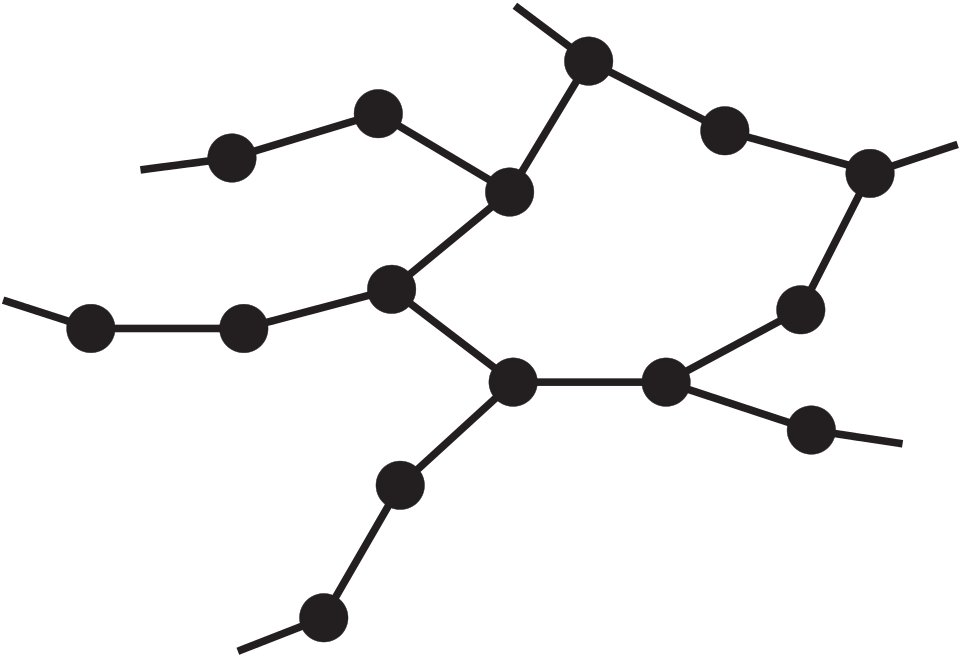
\includegraphics[draft=false,width=0.5\textwidth]{graph.jpg}
\end{minipage}
\pause

\vspace{2ex}
\begin{minipage}[c]{0.35\textwidth}
\begin{itemize}\item Automatic memory management\end{itemize}
\end{minipage} \hspace{1ex}
\begin{minipage}[c]{0.6\textwidth}
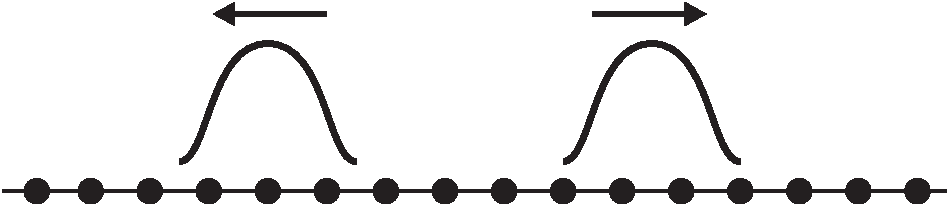
\includegraphics[draft=false,width=0.9\textwidth]{self_expanding_lattice.pdf}

\vspace{0.5ex}
{\scriptsize Enlarge the lattice when waves hit the boundaries}
\end{minipage}
\pause

\vspace{2ex}
\begin{itemize}\item Arbitrary precision types, GMPXX\end{itemize}



\end{frame}


%\section{Technical details}


\begin{frame}
  \tableofcontents[currentsection] 
\end{frame}

\begin{frame}
\heading{Independent Algorithms}
\note{To achive maximum flexibility we wanted to implement the numerical algorithms independent from state type and computation details}

\begin{block}{Goal}
 Container- and computation-independent implementation of the numerical algorithms.  
\end{block}

\begin{block}{Benefit}
 High flexibility and applicability, \odeint\ can be used for virtually any formulation of an ODE.
\end{block}
 
\begin{block}{Approach}
 Detatch the algorithm from memory management and computation details and make each part interchangeable.
\end{block}

\end{frame}

\begin{frame}
\heading{Mathematical Algorithm}

 Typical mathematical computation performed to calculate the solution of an ODE ($\dot{\vec x} = \vec f(\vec x , t)$):

\begin{align*}
 \vec F_1 &= \vec f( \vec x_0 , t_0 ) \\
 \vec x' &= \vec x_0 + a_{21} \cdot \Delta t \cdot \vec F_1 \\ \\
 \vec F_2 &= \vec f( \vec x' , t_0 + c_1\cdot\Delta t ) \\
 \vec x' &= \vec x_0 + a_{31} \cdot \Delta t \cdot \vec F_1 + a_{32} \cdot \Delta t \cdot \vec F_2 \\
         &\vdots \\
 \vec x_1 &= \vec x_0 + b_1\cdot \Delta t \cdot \vec F_1 + \dots + b_s\cdot \Delta t \cdot \vec F_s
\end{align*} 

\end{frame}

\begin{frame}[fragile]
\heading{Strucutural Requirements}
\begin{align*}
 {\color{red}\vec F_1} &= \vec f( {\color{red}\vec x_0} , {\color{blue}t_0} ) & %\\
 {\color{red}\vec x'} &= {\color{red}\vec x_0} + {\color{dark-green}a_{21}} \cdot {\color{blue}\Delta t} \cdot {\color{red}\vec F_1}
\end{align*}
 
Types:
\begin{itemize}
 \item {\color{red} vector type}, mostly, but not neccessarily, some container like \texttt{vector<double>} {\scriptsize (actually we have \texttt{state\_type} and \texttt{deriv\_type})}
 \item {\color{blue} time type}, usually \texttt{double}
 \item {\color{dark-green} value type}, fundamental arithmetic type
\end{itemize}
\pause
\vspace{0.5em}

Function Call:
\begin{lstlisting}
void rhs( const vector_type &x , vector_type &dxdt , const time_type t )
{ /* user defined */ }

rhs( x0 , F1 , t ); //memory allocation for F1?
\end{lstlisting}
\begin{itemize}
 \item Memory allocation for temporary results (\lstinline+F1+, \lstinline+x'+)
\end{itemize}

\end{frame}


\begin{frame}
 \heading{Computational Requirements}
\begin{align*}
  \vec x_1 = \vec x_0 + b_1\cdot \Delta t \cdot \vec F_1 + \dots + b_s\cdot \Delta t \cdot \vec F_s
\end{align*}

\begin{itemize}
 \item vector-vector addition
 \item scalar-scalar multiplication
 \item scalar-vector multiplication
\end{itemize}
\vspace{2ex}
\centerline{\small $\longrightarrow$ vector space}

\end{frame}

%\subsection{Memory Management}

\begin{frame}[fragile]
 \heading{Type Declarations}

Tell \odeint\ which types your are working with:

\begin{lstlisting}
/* define your types */
typedef vector<double> state_type;
typedef vector<double> deriv_type;
typedef double value_type;
typedef double time_type;

/* define your stepper algorithm */
typedef runge_kutta4< state_type , value_type , deriv_type , time_type > stepper_type;
\end{lstlisting}

Reasonable standard values for the template parameters allows for:

\begin{lstlisting}
typedef runge_kutta4<state_type> stepper_type;
\end{lstlisting}


\end{frame}



\begin{frame}[fragile]
 \heading{Memory Allocation / Resizing}
Two possible situations: dynamic size / fixed size \lstinline+vector_type+
\vspace{0.5em}

\begin{columns}[t]

 \begin{column}{0.5\linewidth}
  \begin{block}{dynamic size - memory allocation required}
   \begin{itemize}
    \item e.g. \lstinline+vector<double>+
    \item declare type as resizeable
    \item specialize resize template
    \item use \lstinline+initially_resizer+, \lstinline+always_resizer+, or \lstinline+never_resizer+ in stepper
   \end{itemize}
  \end{block}
 \end{column}

 \begin{column}{0.5\linewidth}
  \begin{block}{fixed size - memory allocation not required}
   \begin{itemize}
    \item e.g. \lstinline+array<double,N>+
    \item declare type as not resizeable
    \item that's it
   \end{itemize}
  \end{block}
 \end{column}

\end{columns}

\end{frame}

\begin{frame}[fragile]
 \heading{Declare Resizeability}

\begin{lstlisting}
/* by default any type is not resizable */
template< class Container >
struct is_resizeable
{
    typedef boost::false_type type;
    const static bool value = type::value;
};

/* specialization for std::vector */
template< class T, class A >
struct is_resizeable< std::vector< T , A  > >
{
    typedef boost::true_type type;
    const static bool value = type::value;
}; 
\end{lstlisting}
To use a new dynamic sized type, this has to be specialized by the user.
\end{frame}


\begin{frame}[fragile]
\heading{Tell \odeint\ how to resize}
Again: only required if \\
\centerline{\lstinline+is_resizeable<state_type>::type == boost::true_type+.}
\vspace{0.5em}

Class Template responsible for resizing:
\begin{lstlisting}
template< class StateOut , class StateIn >
struct resize_impl
{
    /* standard implementation */
    static void resize( StateOut &x1 , const StateIn &x2 )
    {
        x1.resize( boost::size( x2 ) );
    }
};
\end{lstlisting}

For anything that does not support \lstinline+boost::size+ and/or \lstinline+resize+ the user must provide a specialization.

\end{frame}


\begin{frame}[fragile]
 \heading{Tell odeint when to resize}
\vspace{2ex}

\begin{lstlisting}
typedef initially_resizer resizer; //default
\end{lstlisting}
Resizing only at first step (memory allocation)

\vspace{1ex}
\begin{lstlisting}
typedef always_resizer resizer;
\end{lstlisting}
Resizing at every step (expanding lattice)

\vspace{1ex}
\begin{lstlisting}
typedef never_resizer resizer;
\end{lstlisting}
Resizing manually by the user (\lstinline+stepper.adjust_size+)

\vspace{2ex}
\begin{lstlisting}
typedef runge_kutta4< state_type , value_type , 
    deriv_type , time_type , algebra , 
    operations , resizer > stepper_type; 
\end{lstlisting}


\end{frame}



\rem{
\begin{frame}[fragile]
 \heading{Scalar Computations}

For the scalar types we require the following:

Assume:
\begin{lstlisting}
time_type t , dt;
value_type a1 , a2 , c;
\end{lstlisting}

Valid Expressions:
\begin{itemize}
 \item \lstinline+a1 = static_cast< value_type >(1)+
 \item \lstinline+a1*a2+, \lstinline+a1/a2+, \lstinline!a1+a2!, \lstinline+a1-a2+, \lstinline+-a1+ 
 \item \lstinline!t + c*dt!
 \item \lstinline!t + dt/c!
 \item \lstinline!t += dt!
\end{itemize}

\end{frame}
}

\begin{frame}[fragile]
 \heading{Vector Computations}

\centerline{$\vec x_1 = \vec x_0 + b_1\cdot \Delta t \cdot \vec F_1 + \dots + b_s\cdot \Delta t \cdot \vec F_s$}

\vspace{0.5em}

Split into two parts:

\begin{description}
 \item[1.~Algebra:] responsible for iteration over vector elements
 \item[2.~Operations:] does the mathematical computation on the elements
\end{description}

\vspace{0.5em}

Similar to \lstinline+std::for_each+

\begin{lstlisting}
Algebra algebra;

algebra.for_each3( x1 , x0 , F1 ,
    Operations::scale_sum2( 1.0, b1*dt );
\end{lstlisting}
\pause

The types \lstinline+Algebra+ and \lstinline+Operations+ are template parameters of the steppers, hence exchangeable.
\end{frame}


\begin{frame}[fragile]
 \heading{Vector Computations}

\begin{lstlisting}
state_type x1, x2, ...
algebra_type algebra;
\end{lstlisting}

Algebra has to have defined the following member functions:

\begin{itemize}
 \item \lstinline+algebra.for_each1( x1 , unary_operation );+
 \item \lstinline+algebra.for_each2( x1, x2, binary_operation );+
 \item \lstinline+algebra.for_each3( ... );+

\[\vdots\]

 \item \lstinline+algebra.for_each15( .. , fifteen_ary_op );+
\end{itemize}

\pause
\odeint\ takes the operations from the class \lstinline+Operations+.

\end{frame}

\begin{frame}[fragile]
 \heading{Operations}

\lstinline+Operations+ is a class with the following member classes:
\begin{itemize}
 \item \lstinline+scale+
 \item \lstinline+scale_sum1+
 \item \lstinline+scale_sum2+
% \item \lstinline+scale_sum3+
\[ \vdots \]
 \item \lstinline+scale_sum14+
\end{itemize}

These classes need a constructor and \lstinline+()+-operator that works together with the algebra:
\begin{lstlisting}
value_type b1, b2;
time_type dt;
algebra.for_each3( x1 , x0 , F1 ,
   Operations::scale_sum2( 1.0, b1*dt );
\end{lstlisting}

This computes: $\vec x_1 = 1.0\cdot \vec x_0 + b_1\Delta t\cdot \vec F_1$.
\end{frame}


\begin{frame}[fragile]
 \heading{Example Implementation: \lstinline+range_algebra+ }

\begin{lstlisting}[basicstyle=\scriptsize\ttfamily]
struct range_algebra {
...
 template< class S1 , class S2 , class S3 , class Op >
 static void for_each2( S1 &s1, S2 &s2, S3 &s3, Op op )
 {
   detail::for_each2( boost::begin(s1), boost::end(s1),
                      boost::begin(s2), boost::begin(s3), 
                      op );
 }
...
};

namespace detail {
...
 template< class Iter1, class Iter2, Iter3, class Op >
 void for_each2( Iter1 first1, Iter1 last1, 
                 Iter2 first2, Iter3 first3, Op op )
 {
     for( ; first1 != last1 ; )
         op( *first1++ , *first2++ , *first3++ );
 }
...
};
\end{lstlisting}

\end{frame}


\begin{frame}[fragile]
 \heading{Example Implementation: \lstinline+default_operations+ }
\begin{lstlisting}
template< class Fac1 , class Fac2 >
struct scale_sum2
{
  const Fac1 m_alpha1;
  const Fac2 m_alpha2;

  scale_sum2( Fac1 alpha1 , Fac2 alpha2 ) 
    : m_alpha1( alpha1 ) , m_alpha2( alpha2 ) 
  { }

  template< class T1 , class T2 , class T3 >
  void operator()( T1 &t1 , const T2 &t2 , const T3 &t3 )
  { t1 = m_alpha1 * t2 + m_alpha2 * t3; }

  typedef void result_type;
};
\end{lstlisting}

\end{frame}

\begin{frame}[fragile]

%\lstinline+range_algebra & default_operations+ can be used with any Container that supports Boost.Range and whose \lstinline+container::value_type+ supports operators \lstinline!+,*!.

For example \lstinline+vector< double >+:
\begin{lstlisting}
typedef vector< double > state_type;
typedef vector< double > deriv_type;
typedef double value_type;
typedef double time_type;

typedef runge_kutta4< state_type , value_type , 
                      deriv_type , time_type , 
                      range_algebra , 
                      default_operations 
                    > stepper_type
\end{lstlisting}

\vspace{1em}
As these are also the default values, this can be shortened:
\begin{lstlisting}
typedef runge_kutta4<state_type> stepper_type; 
\end{lstlisting}

\end{frame}


\begin{frame}[fragile]
 \lstinline+range_algebra & default_operations+ work also with

\begin{itemize}
 \item \lstinline+vector< complex<double> >+
 \item \lstinline+list< double >+
 \item \lstinline+array< double , N >+
\end{itemize}

\pause
What about
\begin{itemize}
 \item Ublas \lstinline+vector+
 \item trivial \lstinline+state_type+ like \lstinline+double+
 \item generally: \lstinline+state_type+ that support operators \lstinline!+,*!
\end{itemize}

\vspace{1em}
\centerline{$\longrightarrow$ \lstinline+vector_space_algebra+!}

\end{frame}


\begin{frame}[fragile]
 \heading{\lstinline+vector_space_algebra+}

\begin{lstlisting}
struct vector_space_algebra {
...
 template< class S1 , class S2 , class S3 , class Op >
 static void for_each3( S1 &s1 , S2 &s2 , 
                        S3 &s3 , Op op )
 {
   op( s1 , s2 , s3 );
 }
...
};
\end{lstlisting}

\begin{itemize}
 \item delegates \lstinline+state_type+ directly to the operations 
 \item no iteration
 \item works together with \lstinline+default_operations+ with any \lstinline+state_type+ that supports operators \lstinline!+,*!
\end{itemize}

\end{frame}


\begin{frame}[fragile]
 \heading{Other Examples}

\begin{description}
 \item[fusion\_algebra:] works with compile-time sequences like \lstinline+fusion::vector+ of Boost.Units
 \item[thrust\_algebra \& thrust\_operations:] Use thrust library to perform computation on CUDA graphic cards
 \item[mkl\_operations:] Use Intel's Math Kernel Library
 %\item[nested\_algebra:] can handle nested containers that support Boost.Range, e.g.\ \lstinline+vector< vector<double> >+
\end{description}

See tutorial and documentation on \verb+www.odeint.com+ for more.

\pause
\vspace{0.5em}
\begin{block}{Important}
 Division into Algebra and Operations gives us great flexibility. However, state type, algebra and operations must coorporate to make \odeint\ work!
\end{block}

\end{frame}

\begin{frame}
 \heading{More details}

\vspace{2ex}
\begin{itemize}
 \item State wrapper for construction/destruction of state types
 \item More requirements on Algebras when using controlled steppers (\lstinline+algebra.reduce+)
 \item Implicit routines using Ublas
 \item Generation functions to create controlled / dense output steppers
 \item TMP Runge-Kutta implementation (see my talk on Thursday afternoon!)
\end{itemize}

\end{frame}



\section{Conclusion and Discussion}

\begin{frame}
  \tableofcontents[currentsection] 
\end{frame}


\begin{frame}[fragile]
 \heading{Conclusion}

\vspace{2ex}

odeint is a modern C++ library for solving ODEs that is
%odeint is a modern C++ library for solving ordinary differential equations, which is

\begin{itemize}
 \item easy-to-use
 \item highly-flexible
 \begin{itemize}
  \item data types (topology of the ODE, complex numbers, precision, \dots)
  \item computations (CPU, CUDA, OpenMP, ...)
 \end{itemize}
 \item fast
\end{itemize}





\end{frame}



\begin{frame}
 \heading{Where can \odeint\ be used?}

 \vspace{2ex}

 \begin{itemize}
  \item Science
  \item Game engine and physics engines
  \item Simulations
  \item Modelling
  \item Data analysis
  \item High performance computing
 \end{itemize}

\end{frame}


\rem{
\begin{frame}[fragile]
 
 \heading{Who uses odeint}

\vspace{4ex}



\begin{minipage}{0.2\textwidth}
 \begin{center}
  NetEvo

  \vspace{1ex}
  
  
\includegraphics[draft=false,width=1.0\textwidth]{netevo.png}
 \end{center}
\end{minipage}
\hspace{2ex}\begin{minipage}{0.3\textwidth}
 \begin{center}
  \textbf{OMPL} -- Open Motion Planning Library
 \end{center}
\end{minipage}
\hspace{2ex}\begin{minipage}{0.3\textwidth}
 \begin{center}
   \textbf{icicle} -- cloud/precipitation model
 \end{center}
\end{minipage}


\end{frame}
}

\begin{frame}[fragile]
 
 \heading{Who uses odeint}

\vspace{2ex}


\textbf{NetEvo} -- Simulation dynamical networks

\vspace{2ex}
\textbf{OMPL} -- Open Motion Planning Library

\vspace{2ex}
\textbf{icicle} -- cloud/precipitation model

\vspace{2ex}
\textbf{Score} -- Commercial Smooth Particle Hydrodynamics Simulation

\vspace{2ex}
\textbf{VLE} -- Virtual Environment Laboratory (planned to use \odeint )

\vspace{2ex}
Several research groups

\vspace{2ex}
\dots


\end{frame}




\begin{frame}
 \heading{Who uses MTL4}
  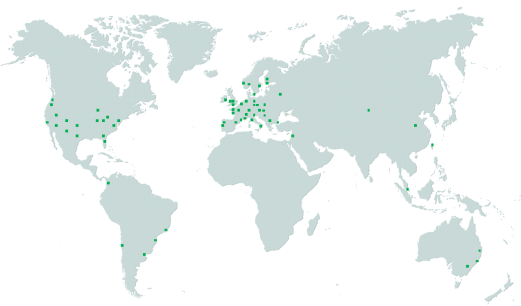
\includegraphics[width=1.0\columnwidth]{MTL4_worldwide}
  \vspace{-6.5cm} 
  \begin{itemize}
  \item \pause  %\color{simuorange}
    FEniCS: free software for automatic PDE solving.%\pause
    \begin{itemize}
    \item %\color{simuorange}
      University of Chicago, Argonne National
      Laboratory, Delft University of Technology, Royal Institute of
      Technology KTH, Simula Research Laboratory, Texas Tech
      University und University of Cambridge.%\pause
    \end{itemize}
  \item Halcrow Yolles (UK): solution of architectural problems in highly complex geometries.%\pause
  \item Institut Fran�ais du P�trole: multi-phase simulation of CO${}_2$ storage by finite volumes.%\pause
  \item Sarturis: interactive simulation of construction machines (virtual reality).%\pause
  \item Serbian Institute for groundwater resources.%\pause
   \item ViennaCL: OpenCL-algebra lib by Vienna university
  \end{itemize}
\end{frame}



\rem{
\begin{frame}
 \heading{Roadmap}

 \vspace{2ex}

Near future:
\begin{itemize}
\item Current release -- documentation, bug fixing
\item \sout{Boost Review process}
\item Implicit steppers
\end{itemize}

\vspace{2ex}
Further plans 
\begin{itemize}
 \item Dormand-Prince 853 steppers
 \item More algebras: MPI, cublas, TBB, John Maddock's arbitrary precision library, Boost SIMD library
\end{itemize}

\vspace{2ex}                                                                                                       
Perspective
\begin{itemize}
 \item C++11 version
 \item sdeint -- methods for stochastic differential equations
 \item ddeint -- methods for delay differential equations
\end{itemize}




\end{frame}
}

\begin{frame}

\heading{THANK YOU!}

\end{frame}


%\begin{frame}
 \centerline{\Large Old Stuff}
\end{frame}



\frame{
  \frametitle{First example -- Lorenz system}
  \lstinputlisting{snippets/example1_a.cpp}

  \begin{itemize}
  \item The r.h.s. of the ODE is a simple function
  \item Observer
  \end{itemize}
}

\begin{frame}[fragile]{Lorenz system continued}
  % \lstinputlisting{snippets/example1_b.cpp}

  Different steppers:

  \begin{lstlisting}
runge_kutta4< state_type > stepper;
  \end{lstlisting}

  \pause
  
  \begin{lstlisting}
controlled_runge_kutta< runge_kutta_cash_karp54< state_type > > stepper;
  \end{lstlisting}

  \pause

  \begin{lstlisting}
dense_output_runge_kutta< controlled_runge_kutta<
    runge_kutta_dopri5< state_type > > > stepper;
  \end{lstlisting}

  \pause

  \begin{lstlisting}
runge_kutta_dopri5< state_type > stepper;
make_dense_output( 1.0e-6 , 1.0e-6 , stepper );    // incomplete
  \end{lstlisting}

  \pause

  All together:

  \begin{lstlisting}
int main( int argc , char **argv )
{
    state_type x = {{ 10.0 , 1.0 , 1.0 }};
    runge_kutta_dopri5< state_type > stepper;
    integrate_const( make_dense_output( 1.0e-6 , 1.0e-6 , stepper )
                     lorenz , x , 0.0 , 10.0 , 0.01 , write_lorenz );
    return 0;
}
  \end{lstlisting}



  
\end{frame}

\rem{
\frame{
  \frametitle{Side note: Templates}

  \begin{itemize}
  \item Programming paradigm: Generic programming
  \item Provide a mechanism that classes and functions work on arbitrary types
  \item Static (compile-time) polymorphism
  \item Good performance -- Compiler can optimize
  \item No virtual functions and runtime-polymorphy in odeint
  \item Concepts -- Description of requirements on the used types and classes
  \item Disadvantage: Long compilation time and memory consumption of the compiler
  \end{itemize}
}
}



\begin{frame}[fragile]{Second example -- Fermi-Pasta-Ulam lattice}
 
  \vspace{-4ex} 
 
  \begin{eqnarray}
   \dot{q}_k & = & p_k  \nonumber \\
   \dot{p}_k & = & - q_k^2 + \Delta q_k + \beta \big\{ ( q_{k+1} - q_k )^3 - ( q_k - q_{k-1} )^3 \big\} \nonumber
  \end{eqnarray}

  \centerline{\rem{Discrete Laplacian} $\Delta q_k = q_{k+1} -2 q_k + q_{k-1}$}

  \vspace{4ex}

  \pause

State type consists of coordinates $q$ and momentas $p$

  \vspace{1ex}

  \begin{lstlisting}
typedef std::vector<double> vector_type;
vector_type q( 256 ) , p( 256 );
// initialize q,p
std::pair< state_type , state_type > state = std::make_pair( q , p );
  \end{lstlisting}

  \pause

  \vspace{2ex}

  Hamiltonian system $\Longrightarrow{}$ Symplectic solvers needed

  \vspace{1ex}

  \begin{lstlisting}
symplectic_rkn_sb3a_mclachlan< vector_type > stepper;
  \end{lstlisting}


\end{frame}

\begin{frame}[fragile]{Fermi-Pasta-Ulam lattice continued}

  Trivial first component $\dot{q}_k = p_k$

  \begin{lstlisting}
struct fpu {
    double m_beta;
    fpu(double beta) : m_beta(beta) { }

    void operator()(const vector_type &q, vector_type &dpdt) const {
        // ...
    }
};
  \end{lstlisting}

  \pause

  \vspace{2ex}

  All together

  \begin{lstlisting}
struct statistics_observer {
    void operator()( const state_type &x , double t ) const { 
    // write the statistics
    }
};

int main(int argc, char **argv)
{
    vector_type q( 256 ) , p( 256 );
    // initialize q,p
    integrate_const( symplectic_rkn_sb3a_mclachlan< state_type >(), fpu(1.0),
        make_pair( q , p ), 0.0, 10.0, 0.01, statistics_observer() );
    return 0;
}
  \end{lstlisting}



\end{frame}



%\section{odeint details}

\frame{\tableofcontents[currentsection]}


\frame{
  \frametitle{Structure of odeint}

  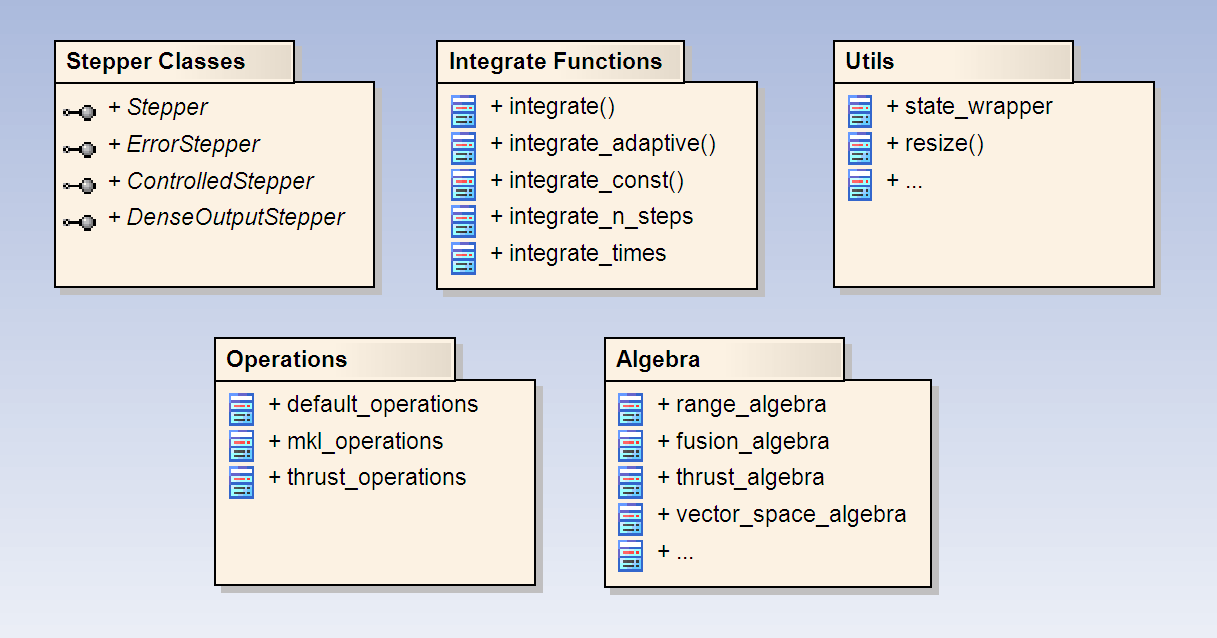
\includegraphics[draft=false,width=1.0\textwidth]{odeint_components.png}

}



\begin{frame}[fragile]
  \frametitle{Internals -- Example Euler's method}

User provides 
  \begin{displaymath}
    y_i = f_i( x(t) , t ) % \,\,\textrm{,} \quad \textrm{for all} \quad i \in (1,\dots,N)
  \end{displaymath}

odeint provides
  \begin{displaymath}
    x_i (t + \Delta t ) = x_i( t )  + \Delta t \cdot y_i
  \end{displaymath}

(In general vector operations like $\,\, z_i = a_1 x_{1,i} + a_2 x_{2,i} + \dots $)



\vspace{4ex}

Instantiation

\vspace{1ex}

\begin{lstlisting}[basicstyle=\small\ttfamily,escapechar=!]
euler<state_type, value_type, deriv_type, time_type, algebra, operations > stepper;
\end{lstlisting}

\vspace{1ex}

{\bf All elements for container independence and portability are already included in this line!}

\end{frame}

\begin{frame}[fragile]
  \frametitle{Internals -- Example Euler's method}

  \begin{displaymath}
    y_i = f_i( x(t) )
  \end{displaymath}
  \begin{displaymath}
    x_i (t + \Delta t ) = x_i( t )  + \Delta t \cdot y_i
  \end{displaymath}

\vspace{2ex}

\begin{lstlisting}[basicstyle=\small\ttfamily]
euler<state_type, value_type, deriv_type, time_type, algebra, operations > stepper;
\end{lstlisting}

\vspace{2ex}

\begin{overlayarea}{\textwidth}{10cm}
 \rem{\only<1>{General goal: Separation 
  \begin{itemize}
   \item of how an vector is iterated
   \item of how the basic computations are performed
  \end{itemize}
from the stepper
 }}
\rem{ \only<1>{Examples:

  {\tt \scriptsize euler<vector<double>, double, vector<double>, double ,
range\_algebra, default\_operations>;}

\vspace{1ex}

  {\tt \scriptsize euler<vector<complex<double> >, double, vector<complex<double> >, double ,
range\_algebra, default\_operations>;}  

  {\tt \scriptsize euler<thurst::device\_vector<double>, double, thrust::device\_vector<double>, double ,
thrust\_algebra, thrust\_algebra>;} 
}}
 \only<1>{
 Data types
 \begin{itemize}
  \item {\tt state\_type} -- the type of $x$
  \item {\tt value\_type} -- the basic numeric type, e.g. {\tt double}
  \item {\tt deriv\_type} -- the type of $y$
  \item {\tt time\_type} -- the type of $t$, $\Delta t$
 \end{itemize}}
 \only<2>{
 Algebra policies, perform the iteration

 \vspace{2ex}

 Algebra must be a class with public methods
 \begin{itemize}
 \item {\tt for\_each1(x,op)} -- Performs $op(x_i)$ for all $i$
 \item {\tt for\_each2(x1,x2,op)} -- Performs $op(x1_i,x2_i)$ for all $i$
 \item ...
 \end{itemize}}
 \only<3>{
 Operations do the basic computation

 \vspace{2ex}

 Operations must be a class with the public classes (functors)
 \begin{itemize}
 \item {\tt scale\_sum1} -- Calculates $x = a1 \cdot y1 $
 \item {\tt scale\_sum2} -- Calculates $x = a1 \cdot y1 + a2 \cdot y2$
 \item ...
 \end{itemize}}
 \only<4>{
 All together

\vspace{2ex}
   {\tt \scriptsize m\_algebra.for\_each3(xnew ,xold, y ,\\
\hspace{4ex}operations\_type::scale\_sum2<value\_type,time\_type>(1.0,dt));}
}
\end{overlayarea}


\end{frame}




\frame{
  \frametitle{Stepper concepts}

  \begin{block}{Concepts}
    ``... In generic programming, a concept is a description of supported
    operations on a type...''
  \end{block}

  \pause
  \vspace{4ex}
  odeint provides
  \begin{itemize}
   \item Stepper concept \\ \lstinline[basicstyle=\small\ttfamily]+stepper.do_step(sys,x,t,dt);+
   \item ErrorStepper concept \\ \lstinline[basicstyle=\small\ttfamily]+stepper.do_step(sys,x,t,dt,xerr);+
   \item ControlledStepper concept \\ \lstinline[basicstyle=\small\ttfamily]+stepper.try_step(sys,x,t,dt);+
   \item DenseOutputStepper concept \\ \lstinline[basicstyle=\small\ttfamily]+stepper.do_step(sys);+ \\ \lstinline[basicstyle=\small\ttfamily]+stepper.calc_state(t,x);+
  \end{itemize}

}

\rem{
\frame{
  \begin{block}{Concepts}
    ``... In generic programming, a concept is a description of supported
    operations on a type...''
  \end{block}
  \begin{columns}[t]
    \begin{column}{0.32\textwidth}
      \begin{block}{Stepper}
        {\footnotesize
          provides method:
          {do\_step(sys,x,t,dt)}

        \vspace{1ex}

        Performs one time step with constant step size

        \vspace{1ex}

        Example:

        stepper\_rk4<vector>~rk;

        ...

        rk.do\_step(lor,x,t,dt);
        }
      \end{block}
    \end{column}
    \begin{column}{0.32\textwidth}
      \begin{block}{Error stepper}
        {\footnotesize
          provides method:
          {do\_step(sys,x,t,dt,xerr)}

        \vspace{1ex}

        Performs one time step with constant step size and error estimation

        \vspace{1ex}

        Example:

        stepper\_rk5\_ck<..>~rk;

        ...

        rk.do\_step(lor,x,t,dt,xerr);}
      \end{block}
    \end{column}
    \begin{column}{0.32\textwidth}
      \begin{block}{Controlled stepper}
        {\footnotesize
          provides method:
          {try\_step(sys,x,t,dt)}

        \vspace{1ex}

        Tries to performs one time step within a given accuracy. Suggests new
        step size.

        \vspace{1ex}

        Example:

        controlled\_stepper\_bs;
        }
      \end{block}
    \end{column}
  \end{columns}

  Dense output concept
}
}

\frame{
  \frametitle{Supported methods}
    {\scriptsize
    \begin{tabular}{lll}
      {\bf Method} & {\bf Class name} & {\bf Concept} \\
      Euler & {\tt euler} & SD \\
      Runge-Kutta 4 & {\tt runge\_kutta4} & S \\
      Runge-Kutta Cash-Karp & {\tt runge\_kutta\_cash\_karp54} & SE \\
      Runge-Kutta Fehlberg & {\tt runge\_kutta\_runge\_fehlberg78} & SE \\
      Runge-Kutta Dormand-Prince & {\tt runge\_kutta\_dopri5} & SED \\
      & & \\
      Runge-Kutta controller & {\tt controlled\_runge\_kutta} & C \\
      Runge-Kutta dense output & {\tt dense\_output\_runge\_kutta} & D \\
      & & \\
      Symplectic Euler & {\tt symplectic\_euler} & S \\
      Symplectic RKN & {\tt symplectic\_rkn\_sb3a\_mclachlan} & S \\
      & & \\
      Rosenbrock 4 & {\tt rosenbrock4} & ECD \\
      Implicit Euler & {\tt implicit\_euler} & S \\
      & & \\
      Adams-Bashforth-Moulton & {\tt adams\_bashforth\_moulton} & S \\
      Bulirsch-Stoer & {\tt bulirsch\_stoer} & CD 
    \end{tabular}

    \vspace{4ex}

    S -- fulfills stepper concept

    E -- fulfills error stepper concept

    C -- fulfills controlled stepper concept

    D -- fulfills dense output stepper concept

  }
}






\frame{
  \frametitle{Integrate functions}

  \begin{itemize}
   \item {\tt integrate\_const}
   \item {\tt integrate\_adaptive}
   \item {\tt integrate\_times}
   \item {\tt integrate\_n\_steps}
  \end{itemize}

  Perform many steps, use all features of the underlying method

  \vspace{2ex}

  \pause

  An additional observer can be called

  \vspace{2ex}

  {\tt integrate\_const(stepper, sys, x, t\_start, t\_end, dt, obs);}

}





\frame{
  \frametitle{More internals}
    \begin{itemize}
      \item Header-only, no linking $\rightarrow$ powerful compiler optimization
      \item Memory allocation is managed internally
      \item No virtual inheritance, no virtual functions are called
      \item Different container types are supported, for example
        \begin{itemize}
          \item STL containers ({\tt vector}, {\tt list}, {\tt map}, {\tt tr1::array})
          \item MTL4 matrix types, blitz++ arrays, Boost.Ublas matrix types
          \item {\tt thrust::device\_vector}
          \item Fancy types, like Boost.Units
          \item ANY type you like
        \end{itemize}
      \item Explicit Runge-Kutta-steppers are implemented with a new template-metaprogramming method
      \item Different operations and algebras are supported
        \begin{itemize}
          \item MKL
          \item Thrust
          \item gsl
        \end{itemize}
    \end{itemize}
}


\frame{
  \frametitle{ODEs on GPUs}

  Graphical processing units (GPUs) are able to perform up to $10^6$ operations at once in parallel
 
  \vspace{2ex}

  Frameworks
  \begin{itemize}
   \item CUDA from NVIDIA
   \item OpenCL
   \item Thrust a STL-like library for CUDA and OpenMP
  \end{itemize}

  \vspace{2ex}

  Applications:
  \begin{itemize}
   \item Parameter studies
   \item Large systems, like ensembles or one- or two dimensional lattices
   \item Discretizations of PDEs
  \end{itemize}

  \vspace{2ex}

  {\bf odeint supports CUDA, through Thrust}
}

\frame{
  \frametitle{Example: Parameter study of the Lorenz system}

  \lstinputlisting{snippets/example3_thrust.cpp}
}




%\section{Outlook and conclusion}

\frame{
  \frametitle{Conclusion}

  \begin{itemize}
    \item odeint provides a fast, flexible and easy-to-use C++ library for
      numerical integration of ODEs.
    \item Its container independence is a large advantage over existing
      libraries.
    \item Portable
    \item Generic programming is the main programming technique.
  \end{itemize}

}



\frame{
  \frametitle{Outlook}
  \begin{itemize}
    \item Submission to the boost libraries
    \item Dynamical system classes for easy implementation of interacting dynamical systems
    \item More methods: implicit methods and multistep methods.
    \item Implementation of the Taylor series method
  \end{itemize}

  \vspace{4ex}

  \lstinputlisting{snippets/example4_lorenz_taylor.cpp}
}



\frame{
  \frametitle{Resources}

Download and documentation

{\tt odeint.com}

\vspace{2ex}

An article about the used techniques exists at

{\tt \small http://www.codeproject.com/KB/recipes/odeint-v2.aspx}

\vspace{2ex}

Development

{\tt https://github.com/headmyshoulder/odeint-v2}

\vspace{4ex}

\begin{block}{Contributions and feedback}
 are highly welcome
\end{block}





}

}


\end{document}
